\INEchaptercarta{Alumnos en básico}{}



\cajita{Inscritos en básico }{El número de  inscritos en básico, se obtiene a partir del total de los alumnos registrados al treinta de marzo de cada año escolar y que comprenden de trece a quince años. \\ 
	
	 En la presente gráfica en serie de años, se observa que en el año 2009 se inscribieron 671,872 alumnos y en el año 2013 se inscribieron 764,415 alumnos, lo cual muestra un crecimiento de 13.8\%.}{Número de inscritos en el ciclo de educación básica}{República de Guatemala, serie histórica, en datos absolutos}{\ \\[0mm]\begin{tikzpicture}[x=1pt,y=1pt]  % Created by tikzDevice version 0.7.0 on 2015-09-01 14:15:14
% !TEX encoding = UTF-8 Unicode
\definecolor[named]{fillColor}{rgb}{1.00,1.00,1.00}
\path[use as bounding box,fill=fillColor,fill opacity=0.00] (0,0) rectangle (289.08,198.74);
\begin{scope}
\path[clip] (  0.00,  0.00) rectangle (289.08,198.74);
\definecolor[named]{drawColor}{rgb}{1.00,1.00,1.00}

\path[draw=drawColor,line width= 0.6pt,line join=round,line cap=round] (  0.00,  0.00) rectangle (289.08,198.74);
\end{scope}
\begin{scope}
\path[clip] (  0.00,  0.00) rectangle (289.08,198.74);

\path[] ( -2.73, 17.78) rectangle (280.54,191.48);

\path[] (  0.00, 53.87) --
	(280.54, 53.87);

\path[] (  0.00,110.27) --
	(280.54,110.27);

\path[] (  0.00,166.67) --
	(280.54,166.67);

\path[] (  0.00, 25.67) --
	(280.54, 25.67);

\path[] (  0.00, 82.07) --
	(280.54, 82.07);

\path[] (  0.00,138.47) --
	(280.54,138.47);

\path[] ( 29.95, 17.78) --
	( 29.95,191.48);

\path[] ( 84.43, 17.78) --
	( 84.43,191.48);

\path[] (138.90, 17.78) --
	(138.90,191.48);

\path[] (193.38, 17.78) --
	(193.38,191.48);

\path[] (247.86, 17.78) --
	(247.86,191.48);
\definecolor[named]{drawColor}{rgb}{0.00,0.00,1.00}

\path[draw=drawColor,line width= 1.7pt,line join=round] ( 29.95,183.59) --
	( 84.43,169.49) --
	(138.90,166.67) --
	(193.38,149.75) --
	(247.86,127.19);
\definecolor[named]{drawColor}{rgb}{0.00,0.00,0.00}

\node[text=drawColor,anchor=base,inner sep=0pt, outer sep=0pt, scale=  1.01] at ( 29.95,187.54) {5.6};

\node[text=drawColor,anchor=base west,inner sep=0pt, outer sep=0pt, scale=  1.01] at ( 84.43,173.44) {5.1};

\node[text=drawColor,anchor=base west,inner sep=0pt, outer sep=0pt, scale=  1.01] at (138.90,170.62) {5.0};

\node[text=drawColor,anchor=base west,inner sep=0pt, outer sep=0pt, scale=  1.01] at (193.38,153.70) {4.4};

\node[text=drawColor,anchor=base,inner sep=0pt, outer sep=0pt, scale=  1.01] at (247.86,115.32) {3.6};
\definecolor[named]{fillColor}{rgb}{0.00,0.00,0.00}

\path[draw=drawColor,line width= 0.1pt,line join=round,fill=fillColor] (  0.00, 25.67) -- (280.54, 25.67);
\end{scope}
\begin{scope}
\path[clip] (  0.00,  0.00) rectangle (289.08,198.74);

\path[] (  0.00, 17.78) --
	(280.54, 17.78);
\end{scope}
\begin{scope}
\path[clip] (  0.00,  0.00) rectangle (289.08,198.74);

\path[] ( 29.95, 13.51) --
	( 29.95, 17.78);

\path[] ( 84.43, 13.51) --
	( 84.43, 17.78);

\path[] (138.90, 13.51) --
	(138.90, 17.78);

\path[] (193.38, 13.51) --
	(193.38, 17.78);

\path[] (247.86, 13.51) --
	(247.86, 17.78);
\end{scope}
\begin{scope}
\path[clip] (  0.00,  0.00) rectangle (289.08,198.74);
\definecolor[named]{drawColor}{rgb}{0.00,0.00,0.00}

\node[text=drawColor,anchor=base,inner sep=0pt, outer sep=0pt, scale=  1.00] at ( 29.95,  2.85) {1987};

\node[text=drawColor,anchor=base,inner sep=0pt, outer sep=0pt, scale=  1.00] at ( 84.43,  2.85) {1995};

\node[text=drawColor,anchor=base,inner sep=0pt, outer sep=0pt, scale=  1.00] at (138.90,  2.85) {1998/99};

\node[text=drawColor,anchor=base,inner sep=0pt, outer sep=0pt, scale=  1.00] at (193.38,  2.85) {2002};

\node[text=drawColor,anchor=base,inner sep=0pt, outer sep=0pt, scale=  1.00] at (247.86,  2.85) {2008/09};
\end{scope}
  \end{tikzpicture}}{Instituto Nacional de Estadística}

\cajita{Inscritos en básico por sexo}{En la presente gráfica, se observa que el porcentaje de hombres inscritos en básico es 53.7\% y de mujeres  46.3\% siendo la diferencia de 7.4 puntos porcentuales.}{Distribución de inscritos en el ciclo de educación básica, por sexo}{República de Guatemala, año 2013, en porcentaje}{\ \\[0mm]\begin{tikzpicture}[x=1pt,y=1pt]  % Created by tikzDevice version 0.7.0 on 2015-08-28 13:12:34
% !TEX encoding = UTF-8 Unicode
\definecolor[named]{fillColor}{rgb}{1.00,1.00,1.00}
\path[use as bounding box,fill=fillColor,fill opacity=0.00] (0,0) rectangle (289.08,198.74);
\begin{scope}
\path[clip] ( 30.54,  0.00) rectangle (258.54,198.74);
\definecolor[named]{drawColor}{rgb}{1.00,1.00,1.00}

\path[draw=drawColor,line width= 0.6pt,line join=round,line cap=round] ( 30.54,  0.00) rectangle (258.54,198.74);
\end{scope}
\begin{scope}
\path[clip] (  0.00,  0.00) rectangle (289.08,198.74);

\path[] (  9.28,  7.11) rectangle (200.91,198.74);

\path[] (105.09,102.93) --
	(191.31,101.55);

\path[] (105.09,102.93) --
	( 18.87,104.30);

\path[] (105.09,102.93) --
	(106.47,189.15);

\path[] (105.09,102.93) --
	(191.31,101.55);

\path[] (105.09,102.93) --
	(103.72, 16.71);

\path[] (105.09,102.93) --
	( 18.87,104.30);

\path[] (105.09,102.93) --
	(105.09,102.93) --
	(105.09,102.93) --
	(105.09,102.93) --
	(105.09,102.93) --
	(105.09,102.93) --
	(105.09,102.93) --
	(105.09,102.93) --
	(105.09,102.93) --
	(105.09,102.93) --
	(105.09,102.93) --
	(105.09,102.93) --
	(105.09,102.93) --
	(105.09,102.93) --
	(105.09,102.93) --
	(105.09,102.93) --
	(105.09,102.93) --
	(105.09,102.93) --
	(105.09,102.93) --
	(105.09,102.93) --
	(105.09,102.93) --
	(105.09,102.93) --
	(105.09,102.93) --
	(105.09,102.93) --
	(105.09,102.93) --
	(105.09,102.93) --
	(105.09,102.93) --
	(105.09,102.93) --
	(105.09,102.93) --
	(105.09,102.93) --
	(105.09,102.93) --
	(105.09,102.93) --
	(105.09,102.93) --
	(105.09,102.93) --
	(105.09,102.93) --
	(105.09,102.93) --
	(105.09,102.93) --
	(105.09,102.93) --
	(105.09,102.93) --
	(105.09,102.93) --
	(105.09,102.93) --
	(105.09,102.93) --
	(105.09,102.93) --
	(105.09,102.93) --
	(105.09,102.93) --
	(105.09,102.93) --
	(105.09,102.93) --
	(105.09,102.93) --
	(105.09,102.93) --
	(105.09,102.93) --
	(105.09,102.93) --
	(105.09,102.93) --
	(105.09,102.93) --
	(105.09,102.93) --
	(105.09,102.93) --
	(105.09,102.93) --
	(105.09,102.93) --
	(105.09,102.93) --
	(105.09,102.93) --
	(105.09,102.93) --
	(105.09,102.93) --
	(105.09,102.93) --
	(105.09,102.93) --
	(105.09,102.93) --
	(105.09,102.93) --
	(105.09,102.93) --
	(105.09,102.93) --
	(105.09,102.93) --
	(105.09,102.93) --
	(105.09,102.93) --
	(105.09,102.93) --
	(105.09,102.93) --
	(105.09,102.93) --
	(105.09,102.93) --
	(105.09,102.93) --
	(105.09,102.93) --
	(105.09,102.93) --
	(105.09,102.93) --
	(105.09,102.93) --
	(105.09,102.93) --
	(105.09,102.93) --
	(105.09,102.93) --
	(105.09,102.93) --
	(105.09,102.93) --
	(105.09,102.93) --
	(105.09,102.93) --
	(105.09,102.93) --
	(105.09,102.93) --
	(105.09,102.93) --
	(105.09,102.93) --
	(105.09,102.93) --
	(105.09,102.93) --
	(105.09,102.93) --
	(105.09,102.93) --
	(105.09,102.93) --
	(105.09,102.93) --
	(105.09,102.93) --
	(105.09,102.93) --
	(105.09,102.93) --
	(105.09,102.93);

\path[] (105.09,122.09) --
	(106.31,122.05) --
	(107.52,121.94) --
	(108.72,121.74) --
	(109.90,121.48) --
	(111.07,121.13) --
	(112.21,120.72) --
	(113.33,120.23) --
	(114.41,119.67) --
	(115.45,119.05) --
	(116.45,118.36) --
	(117.41,117.61) --
	(118.32,116.80) --
	(119.17,115.93) --
	(119.96,115.01) --
	(120.70,114.04) --
	(121.37,113.03) --
	(121.98,111.98) --
	(122.52,110.89) --
	(122.99,109.77) --
	(123.39,108.62) --
	(123.71,107.45) --
	(123.96,106.26) --
	(124.14,105.05) --
	(124.23,103.84) --
	(124.25,102.62) --
	(124.19,101.41) --
	(124.06,100.20) --
	(123.85, 99.00) --
	(123.56, 97.82) --
	(123.20, 96.66) --
	(122.77, 95.52) --
	(122.26, 94.42) --
	(121.69, 93.35) --
	(121.05, 92.31) --
	(120.34, 91.32) --
	(119.57, 90.38) --
	(118.75, 89.49) --
	(117.87, 88.65) --
	(116.94, 87.86) --
	(115.96, 87.14) --
	(114.93, 86.49) --
	(113.87, 85.90) --
	(112.77, 85.37) --
	(111.65, 84.92) --
	(110.49, 84.54) --
	(109.31, 84.24) --
	(108.12, 84.01) --
	(106.91, 83.85) --
	(105.70, 83.77) --
	(104.48, 83.77) --
	(103.27, 83.85) --
	(102.06, 84.01) --
	(100.87, 84.24) --
	( 99.69, 84.54) --
	( 98.54, 84.92) --
	( 97.41, 85.37) --
	( 96.31, 85.90) --
	( 95.25, 86.49) --
	( 94.22, 87.14) --
	( 93.25, 87.86) --
	( 92.31, 88.65) --
	( 91.43, 89.49) --
	( 90.61, 90.38) --
	( 89.84, 91.32) --
	( 89.14, 92.31) --
	( 88.50, 93.35) --
	( 87.92, 94.42) --
	( 87.42, 95.52) --
	( 86.98, 96.66) --
	( 86.62, 97.82) --
	( 86.33, 99.00) --
	( 86.12,100.20) --
	( 85.99,101.41) --
	( 85.93,102.62) --
	( 85.95,103.84) --
	( 86.05,105.05) --
	( 86.22,106.26) --
	( 86.47,107.45) --
	( 86.79,108.62) --
	( 87.19,109.77) --
	( 87.66,110.89) --
	( 88.20,111.98) --
	( 88.81,113.03) --
	( 89.48,114.04) --
	( 90.22,115.01) --
	( 91.01,115.93) --
	( 91.87,116.80) --
	( 92.77,117.61) --
	( 93.73,118.36) --
	( 94.73,119.05) --
	( 95.77,119.67) --
	( 96.85,120.23) --
	( 97.97,120.72) --
	( 99.11,121.13) --
	(100.28,121.48) --
	(101.46,121.74) --
	(102.67,121.94) --
	(103.88,122.05) --
	(105.09,122.09);

\path[] (105.09,141.25) --
	(107.52,141.18) --
	(109.94,140.95) --
	(112.34,140.56) --
	(114.72,140.03) --
	(117.05,139.34) --
	(119.34,138.51) --
	(121.56,137.53) --
	(123.72,136.42) --
	(125.81,135.17) --
	(127.81,133.79) --
	(129.73,132.29) --
	(131.54,130.67) --
	(133.24,128.93) --
	(134.84,127.09) --
	(136.31,125.16) --
	(137.66,123.13) --
	(138.87,121.03) --
	(139.95,118.85) --
	(140.89,116.61) --
	(141.69,114.31) --
	(142.34,111.96) --
	(142.83,109.58) --
	(143.18,107.18) --
	(143.37,104.75) --
	(143.41,102.32) --
	(143.30, 99.89) --
	(143.03, 97.47) --
	(142.60, 95.08) --
	(142.03, 92.72) --
	(141.31, 90.39) --
	(140.44, 88.12) --
	(139.43, 85.91) --
	(138.28, 83.76) --
	(137.00, 81.70) --
	(135.59, 79.72) --
	(134.06, 77.83) --
	(132.41, 76.04) --
	(130.65, 74.36) --
	(128.78, 72.80) --
	(126.82, 71.36) --
	(124.78, 70.04) --
	(122.65, 68.86) --
	(120.46, 67.82) --
	(118.20, 66.91) --
	(115.89, 66.15) --
	(113.53, 65.54) --
	(111.15, 65.08) --
	(108.73, 64.78) --
	(106.31, 64.62) --
	(103.88, 64.62) --
	(101.45, 64.78) --
	( 99.04, 65.08) --
	( 96.65, 65.54) --
	( 94.29, 66.15) --
	( 91.98, 66.91) --
	( 89.73, 67.82) --
	( 87.53, 68.86) --
	( 85.40, 70.04) --
	( 83.36, 71.36) --
	( 81.40, 72.80) --
	( 79.54, 74.36) --
	( 77.78, 76.04) --
	( 76.13, 77.83) --
	( 74.59, 79.72) --
	( 73.18, 81.70) --
	( 71.90, 83.76) --
	( 70.75, 85.91) --
	( 69.74, 88.12) --
	( 68.87, 90.39) --
	( 68.15, 92.72) --
	( 67.58, 95.08) --
	( 67.16, 97.47) --
	( 66.89, 99.89) --
	( 66.77,102.32) --
	( 66.81,104.75) --
	( 67.00,107.18) --
	( 67.35,109.58) --
	( 67.85,111.96) --
	( 68.49,114.31) --
	( 69.29,116.61) --
	( 70.23,118.85) --
	( 71.31,121.03) --
	( 72.52,123.13) --
	( 73.87,125.16) --
	( 75.34,127.09) --
	( 76.94,128.93) --
	( 78.64,130.67) --
	( 80.46,132.29) --
	( 82.37,133.79) --
	( 84.37,135.17) --
	( 86.46,136.42) --
	( 88.62,137.53) --
	( 90.85,138.51) --
	( 93.13,139.34) --
	( 95.47,140.03) --
	( 97.84,140.56) --
	(100.24,140.95) --
	(102.66,141.18) --
	(105.09,141.25);

\path[] (105.09,160.42) --
	(108.74,160.30) --
	(112.37,159.95) --
	(115.97,159.38) --
	(119.53,158.57) --
	(123.03,157.55) --
	(126.46,156.30) --
	(129.80,154.84) --
	(133.04,153.16) --
	(136.17,151.29) --
	(139.18,149.22) --
	(142.04,146.97) --
	(144.76,144.53) --
	(147.32,141.93) --
	(149.71,139.18) --
	(151.92,136.27) --
	(153.94,133.24) --
	(155.76,130.08) --
	(157.38,126.81) --
	(158.79,123.44) --
	(159.99,120.00) --
	(160.96,116.48) --
	(161.71,112.91) --
	(162.23,109.30) --
	(162.51,105.66) --
	(162.57,102.02) --
	(162.40, 98.37) --
	(161.99, 94.75) --
	(161.36, 91.15) --
	(160.50, 87.61) --
	(159.42, 84.13) --
	(158.12, 80.72) --
	(156.60, 77.40) --
	(154.88, 74.18) --
	(152.95, 71.08) --
	(150.84, 68.11) --
	(148.54, 65.28) --
	(146.06, 62.60) --
	(143.42, 60.08) --
	(140.63, 57.74) --
	(137.69, 55.58) --
	(134.62, 53.60) --
	(131.43, 51.83) --
	(128.14, 50.26) --
	(124.75, 48.91) --
	(121.29, 47.77) --
	(117.76, 46.85) --
	(114.17, 46.16) --
	(110.56, 45.70) --
	(106.92, 45.47) --
	(103.27, 45.47) --
	( 99.63, 45.70) --
	( 96.01, 46.16) --
	( 92.43, 46.85) --
	( 88.89, 47.77) --
	( 85.43, 48.91) --
	( 82.04, 50.26) --
	( 78.75, 51.83) --
	( 75.56, 53.60) --
	( 72.49, 55.58) --
	( 69.55, 57.74) --
	( 66.76, 60.08) --
	( 64.12, 62.60) --
	( 61.64, 65.28) --
	( 59.34, 68.11) --
	( 57.23, 71.08) --
	( 55.30, 74.18) --
	( 53.58, 77.40) --
	( 52.07, 80.72) --
	( 50.76, 84.13) --
	( 49.68, 87.61) --
	( 48.82, 91.15) --
	( 48.19, 94.75) --
	( 47.78, 98.37) --
	( 47.61,102.02) --
	( 47.67,105.66) --
	( 47.96,109.30) --
	( 48.48,112.91) --
	( 49.22,116.48) --
	( 50.19,120.00) --
	( 51.39,123.44) --
	( 52.80,126.81) --
	( 54.42,130.08) --
	( 56.24,133.24) --
	( 58.26,136.27) --
	( 60.47,139.18) --
	( 62.86,141.93) --
	( 65.42,144.53) --
	( 68.14,146.97) --
	( 71.01,149.22) --
	( 74.01,151.29) --
	( 77.14,153.16) --
	( 80.38,154.84) --
	( 83.72,156.30) --
	( 87.15,157.55) --
	( 90.65,158.57) --
	( 94.21,159.38) --
	( 97.81,159.95) --
	(101.44,160.30) --
	(105.09,160.42);

\path[] (105.09,179.58) --
	(109.95,179.43) --
	(114.79,178.96) --
	(119.60,178.19) --
	(124.34,177.12) --
	(129.01,175.75) --
	(133.58,174.09) --
	(138.04,172.14) --
	(142.36,169.91) --
	(146.53,167.41) --
	(150.54,164.65) --
	(154.36,161.65) --
	(157.99,158.40) --
	(161.40,154.94) --
	(164.58,151.26) --
	(167.53,147.39) --
	(170.22,143.34) --
	(172.66,139.13) --
	(174.82,134.77) --
	(176.70,130.28) --
	(178.29,125.69) --
	(179.58,121.00) --
	(180.58,116.24) --
	(181.27,111.42) --
	(181.66,106.58) --
	(181.73,101.71) --
	(181.50, 96.85) --
	(180.96, 92.02) --
	(180.12, 87.23) --
	(178.97, 82.50) --
	(177.53, 77.86) --
	(175.79, 73.31) --
	(173.77, 68.89) --
	(171.47, 64.60) --
	(168.91, 60.47) --
	(166.09, 56.51) --
	(163.02, 52.73) --
	(159.72, 49.16) --
	(156.20, 45.80) --
	(152.47, 42.68) --
	(148.56, 39.79) --
	(144.47, 37.16) --
	(140.21, 34.80) --
	(135.82, 32.71) --
	(131.31, 30.90) --
	(126.69, 29.38) --
	(121.98, 28.16) --
	(117.20, 27.24) --
	(112.38, 26.62) --
	(107.52, 26.31) --
	(102.66, 26.31) --
	( 97.80, 26.62) --
	( 92.98, 27.24) --
	( 88.20, 28.16) --
	( 83.50, 29.38) --
	( 78.87, 30.90) --
	( 74.36, 32.71) --
	( 69.97, 34.80) --
	( 65.72, 37.16) --
	( 61.62, 39.79) --
	( 57.71, 42.68) --
	( 53.98, 45.80) --
	( 50.46, 49.16) --
	( 47.16, 52.73) --
	( 44.09, 56.51) --
	( 41.27, 60.47) --
	( 38.71, 64.60) --
	( 36.41, 68.89) --
	( 34.39, 73.31) --
	( 32.66, 77.86) --
	( 31.21, 82.50) --
	( 30.06, 87.23) --
	( 29.22, 92.02) --
	( 28.68, 96.85) --
	( 28.45,101.71) --
	( 28.53,106.58) --
	( 28.91,111.42) --
	( 29.60,116.24) --
	( 30.60,121.00) --
	( 31.90,125.69) --
	( 33.49,130.28) --
	( 35.37,134.77) --
	( 37.53,139.13) --
	( 39.96,143.34) --
	( 42.65,147.39) --
	( 45.60,151.26) --
	( 48.78,154.94) --
	( 52.20,158.40) --
	( 55.82,161.65) --
	( 59.64,164.65) --
	( 63.65,167.41) --
	( 67.82,169.91) --
	( 72.15,172.14) --
	( 76.60,174.09) --
	( 81.17,175.75) --
	( 85.84,177.12) --
	( 90.58,178.19) --
	( 95.39,178.96) --
	(100.23,179.43) --
	(105.09,179.58);

\path[] (105.09,189.16) --
	(110.56,188.99) --
	(116.01,188.47) --
	(121.41,187.60) --
	(126.75,186.40) --
	(132.00,184.86) --
	(137.14,182.98) --
	(142.15,180.79) --
	(147.02,178.28) --
	(151.71,175.47) --
	(156.22,172.37) --
	(160.52,168.99) --
	(164.60,165.34) --
	(168.44,161.44) --
	(172.02,157.30) --
	(175.33,152.95) --
	(178.37,148.39) --
	(181.10,143.65) --
	(183.53,138.75) --
	(185.65,133.70) --
	(187.44,128.53) --
	(188.89,123.26) --
	(190.01,117.90) --
	(190.79,112.49) --
	(191.23,107.03) --
	(191.31,101.56) --
	(191.05, 96.09) --
	(190.45, 90.66) --
	(189.50, 85.27) --
	(188.21, 79.95) --
	(186.58, 74.72) --
	(184.63, 69.61) --
	(182.36, 64.63) --
	(179.77, 59.81) --
	(176.89, 55.16) --
	(173.71, 50.70) --
	(170.26, 46.46) --
	(166.55, 42.44) --
	(162.59, 38.66) --
	(158.40, 35.14) --
	(153.99, 31.90) --
	(149.39, 28.94) --
	(144.61, 26.28) --
	(139.66, 23.93) --
	(134.58, 21.90) --
	(129.39, 20.19) --
	(124.09, 18.81) --
	(118.72, 17.78) --
	(113.29, 17.09) --
	(107.83, 16.74) --
	(102.36, 16.74) --
	( 96.89, 17.09) --
	( 91.47, 17.78) --
	( 86.09, 18.81) --
	( 80.80, 20.19) --
	( 75.60, 21.90) --
	( 70.52, 23.93) --
	( 65.58, 26.28) --
	( 60.80, 28.94) --
	( 56.19, 31.90) --
	( 51.79, 35.14) --
	( 47.59, 38.66) --
	( 43.63, 42.44) --
	( 39.92, 46.46) --
	( 36.47, 50.70) --
	( 33.30, 55.16) --
	( 30.41, 59.81) --
	( 27.83, 64.63) --
	( 25.55, 69.61) --
	( 23.60, 74.72) --
	( 21.98, 79.95) --
	( 20.69, 85.27) --
	( 19.74, 90.66) --
	( 19.13, 96.09) --
	( 18.87,101.56) --
	( 18.96,107.03) --
	( 19.39,112.49) --
	( 20.17,117.90) --
	( 21.29,123.26) --
	( 22.75,128.53) --
	( 24.54,133.70) --
	( 26.65,138.75) --
	( 29.08,143.65) --
	( 31.82,148.39) --
	( 34.85,152.95) --
	( 38.16,157.30) --
	( 41.74,161.44) --
	( 45.58,165.34) --
	( 49.66,168.99) --
	( 53.96,172.37) --
	( 58.47,175.47) --
	( 63.16,178.28) --
	( 68.03,180.79) --
	( 73.04,182.98) --
	( 78.18,184.86) --
	( 83.43,186.40) --
	( 88.77,187.60) --
	( 94.17,188.47) --
	( 99.62,188.99) --
	(105.09,189.16);
\definecolor[named]{drawColor}{rgb}{1.00,1.00,1.00}
\definecolor[named]{fillColor}{rgb}{0.00,0.00,1.00}

\path[draw=drawColor,line width= 0.6pt,line join=round,line cap=round,fill=fillColor] (103.87, 64.62) --
	(103.78, 61.89) --
	(103.69, 59.15) --
	(103.61, 56.41) --
	(103.52, 53.68) --
	(103.43, 50.94) --
	(103.34, 48.20) --
	(103.26, 45.47) --
	(103.17, 42.73) --
	(103.08, 40.00) --
	(103.00, 37.26) --
	(102.91, 34.52) --
	(102.82, 31.79) --
	(102.73, 29.05) --
	(102.65, 26.32) --
	(102.65, 26.32) --
	(105.26, 26.28) --
	(107.88, 26.33) --
	(110.49, 26.47) --
	(113.09, 26.70) --
	(115.69, 27.01) --
	(118.27, 27.42) --
	(120.84, 27.91) --
	(123.39, 28.49) --
	(125.92, 29.16) --
	(128.43, 29.91) --
	(130.90, 30.75) --
	(133.35, 31.68) --
	(135.77, 32.68) --
	(138.14, 33.77) --
	(140.48, 34.94) --
	(142.78, 36.18) --
	(145.04, 37.51) --
	(147.25, 38.91) --
	(149.41, 40.38) --
	(151.51, 41.93) --
	(153.57, 43.55) --
	(155.57, 45.24) --
	(157.50, 47.00) --
	(159.38, 48.82) --
	(161.20, 50.70) --
	(162.95, 52.65) --
	(164.63, 54.65) --
	(166.24, 56.71) --
	(167.78, 58.82) --
	(169.25, 60.99) --
	(170.64, 63.20) --
	(171.96, 65.46) --
	(173.20, 67.76) --
	(174.36, 70.11) --
	(175.44, 72.49) --
	(176.44, 74.91) --
	(177.35, 77.36) --
	(178.18, 79.84) --
	(178.93, 82.34) --
	(179.59, 84.87) --
	(180.16, 87.43) --
	(180.64, 90.00) --
	(181.04, 92.58) --
	(181.35, 95.18) --
	(181.57, 97.79) --
	(181.70,100.40) --
	(181.74,103.01) --
	(181.70,105.63) --
	(181.56,108.24) --
	(181.33,110.85) --
	(181.02,113.44) --
	(180.62,116.03) --
	(180.12,118.60) --
	(179.55,121.15) --
	(178.88,123.68) --
	(178.13,126.18) --
	(177.29,128.66) --
	(176.37,131.11) --
	(175.37,133.52) --
	(174.29,135.90) --
	(173.12,138.25) --
	(171.88,140.55) --
	(170.55,142.80) --
	(169.16,145.01) --
	(167.68,147.17) --
	(166.14,149.28) --
	(164.52,151.34) --
	(162.83,153.34) --
	(161.08,155.28) --
	(159.26,157.16) --
	(157.38,158.98) --
	(155.44,160.73) --
	(153.44,162.41) --
	(151.38,164.03) --
	(149.27,165.57) --
	(147.10,167.04) --
	(144.89,168.44) --
	(142.63,169.76) --
	(140.33,171.00) --
	(137.99,172.16) --
	(135.61,173.24) --
	(133.19,174.24) --
	(130.74,175.16) --
	(128.26,175.99) --
	(125.76,176.74) --
	(123.23,177.40) --
	(120.68,177.98) --
	(118.11,178.47) --
	(115.52,178.87) --
	(112.92,179.18) --
	(110.32,179.40) --
	(107.71,179.53) --
	(105.09,179.58) --
	(105.09,179.58) --
	(105.09,176.84) --
	(105.09,174.10) --
	(105.09,171.37) --
	(105.09,168.63) --
	(105.09,165.89) --
	(105.09,163.15) --
	(105.09,160.42) --
	(105.09,157.68) --
	(105.09,154.94) --
	(105.09,152.20) --
	(105.09,149.47) --
	(105.09,146.73) --
	(105.09,143.99) --
	(105.09,141.25) --
	(105.09,141.25) --
	(107.73,141.16) --
	(110.36,140.89) --
	(112.97,140.44) --
	(115.53,139.80) --
	(118.05,139.00) --
	(120.51,138.02) --
	(122.89,136.87) --
	(125.19,135.56) --
	(127.39,134.10) --
	(129.48,132.49) --
	(131.46,130.74) --
	(133.32,128.85) --
	(135.04,126.85) --
	(136.62,124.72) --
	(138.04,122.50) --
	(139.31,120.18) --
	(140.42,117.78) --
	(141.36,115.31) --
	(142.13,112.78) --
	(142.72,110.20) --
	(143.13,107.59) --
	(143.36,104.96) --
	(143.41,102.32) --
	(143.28, 99.68) --
	(142.96, 97.05) --
	(142.47, 94.45) --
	(141.80, 91.90) --
	(140.95, 89.39) --
	(139.93, 86.95) --
	(138.75, 84.59) --
	(137.40, 82.32) --
	(135.90, 80.14) --
	(134.26, 78.07) --
	(132.48, 76.12) --
	(130.56, 74.29) --
	(128.53, 72.60) --
	(126.38, 71.06) --
	(124.13, 69.67) --
	(121.80, 68.43) --
	(119.38, 67.36) --
	(116.89, 66.46) --
	(114.35, 65.74) --
	(111.77, 65.19) --
	(109.15, 64.82) --
	(106.51, 64.63) --
	(103.87, 64.62) --
	cycle;
\definecolor[named]{fillColor}{rgb}{0.62,0.73,1.00}

\path[draw=drawColor,line width= 0.6pt,line join=round,line cap=round,fill=fillColor] (105.09,141.25) --
	(105.09,143.99) --
	(105.09,146.73) --
	(105.09,149.47) --
	(105.09,152.20) --
	(105.09,154.94) --
	(105.09,157.68) --
	(105.09,160.42) --
	(105.09,163.15) --
	(105.09,165.89) --
	(105.09,168.63) --
	(105.09,171.37) --
	(105.09,174.10) --
	(105.09,176.84) --
	(105.09,179.58) --
	(105.09,179.58) --
	(102.47,179.53) --
	( 99.86,179.40) --
	( 97.25,179.18) --
	( 94.65,178.86) --
	( 92.06,178.46) --
	( 89.48,177.97) --
	( 86.93,177.40) --
	( 84.40,176.73) --
	( 81.89,175.98) --
	( 79.40,175.15) --
	( 76.95,174.23) --
	( 74.53,173.22) --
	( 72.15,172.14) --
	( 69.80,170.97) --
	( 67.50,169.73) --
	( 65.24,168.40) --
	( 63.02,167.00) --
	( 60.86,165.53) --
	( 58.75,163.98) --
	( 56.69,162.36) --
	( 54.69,160.68) --
	( 52.74,158.92) --
	( 50.86,157.10) --
	( 49.04,155.21) --
	( 47.29,153.27) --
	( 45.60,151.26) --
	( 43.98,149.20) --
	( 42.44,147.09) --
	( 40.97,144.92) --
	( 39.57,142.71) --
	( 38.25,140.44) --
	( 37.01,138.14) --
	( 35.84,135.79) --
	( 34.76,133.41) --
	( 33.76,130.99) --
	( 32.84,128.53) --
	( 32.01,126.05) --
	( 31.26,123.54) --
	( 30.60,121.00) --
	( 30.03,118.45) --
	( 29.54,115.88) --
	( 29.14,113.29) --
	( 28.83,110.69) --
	( 28.61,108.08) --
	( 28.48,105.46) --
	( 28.44,102.84) --
	( 28.49,100.22) --
	( 28.62, 97.61) --
	( 28.85, 95.00) --
	( 29.17, 92.40) --
	( 29.57, 89.81) --
	( 30.06, 87.24) --
	( 30.64, 84.68) --
	( 31.31, 82.15) --
	( 32.06, 79.64) --
	( 32.90, 77.16) --
	( 33.82, 74.71) --
	( 34.83, 72.29) --
	( 35.92, 69.91) --
	( 37.09, 67.56) --
	( 38.33, 65.26) --
	( 39.66, 63.00) --
	( 41.06, 60.79) --
	( 42.54, 58.63) --
	( 44.09, 56.51) --
	( 45.71, 54.46) --
	( 47.40, 52.46) --
	( 49.16, 50.51) --
	( 50.98, 48.63) --
	( 52.87, 46.82) --
	( 54.82, 45.07) --
	( 56.82, 43.38) --
	( 58.89, 41.77) --
	( 61.00, 40.23) --
	( 63.17, 38.76) --
	( 65.39, 37.36) --
	( 67.65, 36.04) --
	( 69.96, 34.80) --
	( 72.31, 33.64) --
	( 74.69, 32.56) --
	( 77.11, 31.56) --
	( 79.57, 30.65) --
	( 82.05, 29.82) --
	( 84.56, 29.08) --
	( 87.10, 28.42) --
	( 89.66, 27.85) --
	( 92.23, 27.36) --
	( 94.82, 26.97) --
	( 97.42, 26.66) --
	(100.03, 26.44) --
	(102.65, 26.32) --
	(102.65, 26.32) --
	(102.73, 29.05) --
	(102.82, 31.79) --
	(102.91, 34.52) --
	(103.00, 37.26) --
	(103.08, 40.00) --
	(103.17, 42.73) --
	(103.26, 45.47) --
	(103.34, 48.20) --
	(103.43, 50.94) --
	(103.52, 53.68) --
	(103.61, 56.41) --
	(103.69, 59.15) --
	(103.78, 61.89) --
	(103.87, 64.62) --
	(103.87, 64.62) --
	(101.23, 64.80) --
	( 98.60, 65.16) --
	( 96.01, 65.69) --
	( 93.46, 66.41) --
	( 90.97, 67.30) --
	( 88.54, 68.36) --
	( 86.19, 69.59) --
	( 83.94, 70.97) --
	( 81.78, 72.51) --
	( 79.73, 74.19) --
	( 77.81, 76.01) --
	( 76.02, 77.96) --
	( 74.36, 80.02) --
	( 72.85, 82.20) --
	( 71.50, 84.48) --
	( 70.31, 86.84) --
	( 69.28, 89.28) --
	( 68.42, 91.78) --
	( 67.74, 94.34) --
	( 67.24, 96.94) --
	( 66.91, 99.57) --
	( 66.77,102.21) --
	( 66.81,104.86) --
	( 67.04,107.50) --
	( 67.45,110.12) --
	( 68.03,112.70) --
	( 68.80,115.24) --
	( 69.73,117.71) --
	( 70.84,120.12) --
	( 72.11,122.44) --
	( 73.53,124.67) --
	( 75.11,126.80) --
	( 76.83,128.81) --
	( 78.68,130.70) --
	( 80.66,132.46) --
	( 82.76,134.08) --
	( 84.97,135.54) --
	( 87.27,136.86) --
	( 89.65,138.01) --
	( 92.11,138.99) --
	( 94.63,139.80) --
	( 97.20,140.43) --
	( 99.81,140.89) --
	(102.44,141.16) --
	(105.09,141.25) --
	cycle;
\definecolor[named]{drawColor}{rgb}{0.00,0.00,0.00}

\node[text=drawColor,anchor=base,inner sep=0pt, outer sep=0pt, scale=  1.00] at (191.31, 97.64) {50.5};

\node[text=drawColor,anchor=base,inner sep=0pt, outer sep=0pt, scale=  1.00] at ( 18.87,100.39) {49.5};
\end{scope}
\begin{scope}
\path[clip] (  0.00,  0.00) rectangle (289.08,198.74);

\path[] (  9.28,  7.11) --
	(  9.28,198.74);
\end{scope}
\begin{scope}
\path[clip] (  0.00,  0.00) rectangle (289.08,198.74);

\path[] (  5.01,102.93) --
	(  9.28,102.93);

\path[] (  5.01,122.09) --
	(  9.28,122.09);

\path[] (  5.01,141.25) --
	(  9.28,141.25);

\path[] (  5.01,160.42) --
	(  9.28,160.42);

\path[] (  5.01,179.58) --
	(  9.28,179.58);
\end{scope}
\begin{scope}
\path[clip] (  0.00,  0.00) rectangle (289.08,198.74);

\path[] (  9.28,  7.11) --
	(200.91,  7.11);
\end{scope}
\coordinate (rect) at (192.72,99.37);
\coordinate (desY) at (0,18.49);
\coordinate (desX) at (7.11,11.38);
\coordinate (mdesX) at (7.11,-11.38);
\definecolor[named]{ct1}{HTML}{
0000FF
}
\definecolor[named]{borde}{HTML}{
0000FF
}
\coordinate (t1) at ($(rect) + 0.5*(desX) + 0.5*(desY)$);
\coordinate (t2) at ($(rect)+0.5*(mdesX)-0.5*(desY)$);
\draw [color=ct1,fill=borde] ($(rect)+(desY)$) rectangle ($(rect)+(desX)$);
\definecolor[named]{ct2}{HTML}{
9DBBFF
}
\node [text width=
56.692913328
,right= 0.3cm of t1,scale = 0.9]{
Hombre
};
\path [fill=ct2] ($(rect)-(desY)$) rectangle ($(rect)+(mdesX)$);
\node [text width=
56.692913328
,right= 0.3cm of t2,scale = 0.9]{
Mujer
};
  \end{tikzpicture}}{Instituto Nacional de Estadística}

\cajita{Inscritos en básico por grado}{En la presente gráfica, se observa el número de inscritos por grado en básico y se observa que donde se concentra la mayor cantidad de alumnos es en primer grado, con el 41.7\% y donde menos inscritos hay, es en tercer grado con 27.9\%.}{Distribución de inscritos en el ciclo de educación básica, según el grado escolar}{República de Guatemala, año 2013, en porcentaje}{\ \\[0mm]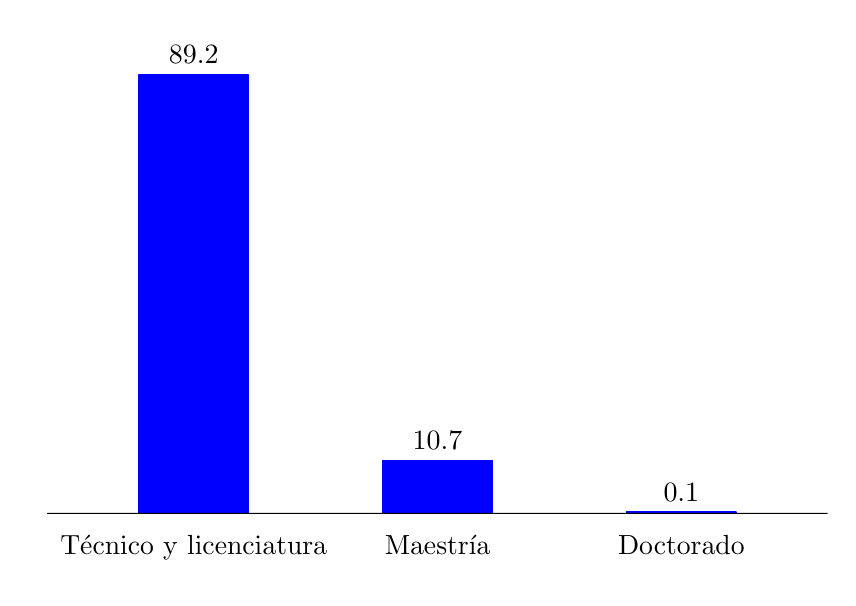
\begin{tikzpicture}[x=1pt,y=1pt]  % Created by tikzDevice version 0.7.0 on 2015-08-28 14:02:54
% !TEX encoding = UTF-8 Unicode
\definecolor[named]{fillColor}{rgb}{1.00,1.00,1.00}
\path[use as bounding box,fill=fillColor,fill opacity=0.00] (0,0) rectangle (289.08,198.74);
\begin{scope}
\path[clip] (  0.00,  0.00) rectangle (289.08,198.74);
\definecolor[named]{drawColor}{rgb}{1.00,1.00,1.00}

\path[draw=drawColor,line width= 0.6pt,line join=round,line cap=round] (  0.00,  0.00) rectangle (289.08,198.74);
\end{scope}
\begin{scope}
\path[clip] (  0.00,  0.00) rectangle (289.08,198.74);

\path[] (  7.11, 23.47) rectangle (289.08,181.67);

\path[] ( 59.98, 23.47) --
	( 59.98,181.67);

\path[] (148.10, 23.47) --
	(148.10,181.67);

\path[] (236.21, 23.47) --
	(236.21,181.67);
\definecolor[named]{drawColor}{rgb}{0.00,0.00,1.00}
\definecolor[named]{fillColor}{rgb}{0.00,0.00,1.00}

\path[draw=drawColor,line width= 0.6pt,line join=round,fill=fillColor] ( 40.16, 23.47) rectangle ( 79.81,181.67);

\path[draw=drawColor,line width= 0.6pt,line join=round,fill=fillColor] (128.27, 23.47) rectangle (167.92, 42.36);

\path[draw=drawColor,line width= 0.6pt,line join=round,fill=fillColor] (216.39, 23.47) rectangle (256.04, 23.73);
\definecolor[named]{drawColor}{rgb}{0.00,0.00,0.00}
\definecolor[named]{fillColor}{rgb}{0.00,0.00,0.00}

\path[draw=drawColor,line width= 0.1pt,line join=round,fill=fillColor] (  7.11, 23.47) -- (289.08, 23.47);

\node[text=drawColor,anchor=base,inner sep=0pt, outer sep=0pt, scale=  1.01] at ( 59.98,185.63) {89.2};

\node[text=drawColor,anchor=base,inner sep=0pt, outer sep=0pt, scale=  1.01] at (148.10, 46.32) {10.7};

\node[text=drawColor,anchor=base,inner sep=0pt, outer sep=0pt, scale=  1.01] at (236.21, 27.68) {0.1};
\end{scope}
\begin{scope}
\path[clip] (  0.00,  0.00) rectangle (289.08,198.74);

\path[] (  7.11, 23.47) --
	(  7.11,181.67);
\end{scope}
\begin{scope}
\path[clip] (  0.00,  0.00) rectangle (289.08,198.74);

\path[] (  7.11, 23.47) --
	(289.08, 23.47);
\end{scope}
\begin{scope}
\path[clip] (  0.00,  0.00) rectangle (289.08,198.74);

\path[] ( 59.98, 19.20) --
	( 59.98, 23.47);

\path[] (148.10, 19.20) --
	(148.10, 23.47);

\path[] (236.21, 19.20) --
	(236.21, 23.47);
\end{scope}
\begin{scope}
\path[clip] (  0.00,  0.00) rectangle (289.08,198.74);
\definecolor[named]{drawColor}{rgb}{0.00,0.00,0.00}

\node[text=drawColor,anchor=base,inner sep=0pt, outer sep=0pt, scale=  1.00] at ( 59.98,  8.54) {T\'ecnico y licenciatura};

\node[text=drawColor,anchor=base,inner sep=0pt, outer sep=0pt, scale=  1.00] at (148.10,  8.54) {Maestr\'ia};

\node[text=drawColor,anchor=base,inner sep=0pt, outer sep=0pt, scale=  1.00] at (236.21,  8.54) {Doctorado};
\end{scope}
  \end{tikzpicture}}{Instituto Nacional de Estadística}

\cajita{Inscritos en básico por etnia}{En la presente gráfica, se observa que del total de inscritos en básico, los no indígenas representan el 75.2\%.}{Distribución de inscritos en el ciclo de educación básica, por grupo étnico}{República de Guatemala, año 2013, en porcentaje}{\ \\[0mm]\begin{tikzpicture}[x=1pt,y=1pt]  % Created by tikzDevice version 0.7.0 on 2015-08-28 13:08:50
% !TEX encoding = UTF-8 Unicode
\definecolor[named]{fillColor}{rgb}{1.00,1.00,1.00}
\path[use as bounding box,fill=fillColor,fill opacity=0.00] (0,0) rectangle (289.08,198.74);
\begin{scope}
\path[clip] ( 30.54,  0.00) rectangle (258.54,198.74);
\definecolor[named]{drawColor}{rgb}{1.00,1.00,1.00}

\path[draw=drawColor,line width= 0.6pt,line join=round,line cap=round] ( 30.54,  0.00) rectangle (258.54,198.74);
\end{scope}
\begin{scope}
\path[clip] (  0.00,  0.00) rectangle (289.08,198.74);

\path[] (  9.28,  7.11) rectangle (200.91,198.74);

\path[] (105.09,102.93) --
	(165.75, 41.64);

\path[] (105.09,102.93) --
	( 44.43,164.22);

\path[] (105.09,102.93) --
	(166.38,163.59);

\path[] (105.09,102.93) --
	(165.75, 41.64);

\path[] (105.09,102.93) --
	( 43.80, 42.27);

\path[] (105.09,102.93) --
	( 44.43,164.22);

\path[] (105.09,102.93) --
	(105.09,102.93) --
	(105.09,102.93) --
	(105.09,102.93) --
	(105.09,102.93) --
	(105.09,102.93) --
	(105.09,102.93) --
	(105.09,102.93) --
	(105.09,102.93) --
	(105.09,102.93) --
	(105.09,102.93) --
	(105.09,102.93) --
	(105.09,102.93) --
	(105.09,102.93) --
	(105.09,102.93) --
	(105.09,102.93) --
	(105.09,102.93) --
	(105.09,102.93) --
	(105.09,102.93) --
	(105.09,102.93) --
	(105.09,102.93) --
	(105.09,102.93) --
	(105.09,102.93) --
	(105.09,102.93) --
	(105.09,102.93) --
	(105.09,102.93) --
	(105.09,102.93) --
	(105.09,102.93) --
	(105.09,102.93) --
	(105.09,102.93) --
	(105.09,102.93) --
	(105.09,102.93) --
	(105.09,102.93) --
	(105.09,102.93) --
	(105.09,102.93) --
	(105.09,102.93) --
	(105.09,102.93) --
	(105.09,102.93) --
	(105.09,102.93) --
	(105.09,102.93) --
	(105.09,102.93) --
	(105.09,102.93) --
	(105.09,102.93) --
	(105.09,102.93) --
	(105.09,102.93) --
	(105.09,102.93) --
	(105.09,102.93) --
	(105.09,102.93) --
	(105.09,102.93) --
	(105.09,102.93) --
	(105.09,102.93) --
	(105.09,102.93) --
	(105.09,102.93) --
	(105.09,102.93) --
	(105.09,102.93) --
	(105.09,102.93) --
	(105.09,102.93) --
	(105.09,102.93) --
	(105.09,102.93) --
	(105.09,102.93) --
	(105.09,102.93) --
	(105.09,102.93) --
	(105.09,102.93) --
	(105.09,102.93) --
	(105.09,102.93) --
	(105.09,102.93) --
	(105.09,102.93) --
	(105.09,102.93) --
	(105.09,102.93) --
	(105.09,102.93) --
	(105.09,102.93) --
	(105.09,102.93) --
	(105.09,102.93) --
	(105.09,102.93) --
	(105.09,102.93) --
	(105.09,102.93) --
	(105.09,102.93) --
	(105.09,102.93) --
	(105.09,102.93) --
	(105.09,102.93) --
	(105.09,102.93) --
	(105.09,102.93) --
	(105.09,102.93) --
	(105.09,102.93) --
	(105.09,102.93) --
	(105.09,102.93) --
	(105.09,102.93) --
	(105.09,102.93) --
	(105.09,102.93) --
	(105.09,102.93) --
	(105.09,102.93) --
	(105.09,102.93) --
	(105.09,102.93) --
	(105.09,102.93) --
	(105.09,102.93) --
	(105.09,102.93) --
	(105.09,102.93) --
	(105.09,102.93) --
	(105.09,102.93) --
	(105.09,102.93);

\path[] (105.09,122.09) --
	(106.31,122.05) --
	(107.52,121.94) --
	(108.72,121.74) --
	(109.90,121.48) --
	(111.07,121.13) --
	(112.21,120.72) --
	(113.33,120.23) --
	(114.41,119.67) --
	(115.45,119.05) --
	(116.45,118.36) --
	(117.41,117.61) --
	(118.32,116.80) --
	(119.17,115.93) --
	(119.96,115.01) --
	(120.70,114.04) --
	(121.37,113.03) --
	(121.98,111.98) --
	(122.52,110.89) --
	(122.99,109.77) --
	(123.39,108.62) --
	(123.71,107.45) --
	(123.96,106.26) --
	(124.14,105.05) --
	(124.23,103.84) --
	(124.25,102.62) --
	(124.19,101.41) --
	(124.06,100.20) --
	(123.85, 99.00) --
	(123.56, 97.82) --
	(123.20, 96.66) --
	(122.77, 95.52) --
	(122.26, 94.42) --
	(121.69, 93.35) --
	(121.05, 92.31) --
	(120.34, 91.32) --
	(119.57, 90.38) --
	(118.75, 89.49) --
	(117.87, 88.65) --
	(116.94, 87.86) --
	(115.96, 87.14) --
	(114.93, 86.49) --
	(113.87, 85.90) --
	(112.77, 85.37) --
	(111.65, 84.92) --
	(110.49, 84.54) --
	(109.31, 84.24) --
	(108.12, 84.01) --
	(106.91, 83.85) --
	(105.70, 83.77) --
	(104.48, 83.77) --
	(103.27, 83.85) --
	(102.06, 84.01) --
	(100.87, 84.24) --
	( 99.69, 84.54) --
	( 98.54, 84.92) --
	( 97.41, 85.37) --
	( 96.31, 85.90) --
	( 95.25, 86.49) --
	( 94.22, 87.14) --
	( 93.25, 87.86) --
	( 92.31, 88.65) --
	( 91.43, 89.49) --
	( 90.61, 90.38) --
	( 89.84, 91.32) --
	( 89.14, 92.31) --
	( 88.50, 93.35) --
	( 87.92, 94.42) --
	( 87.42, 95.52) --
	( 86.98, 96.66) --
	( 86.62, 97.82) --
	( 86.33, 99.00) --
	( 86.12,100.20) --
	( 85.99,101.41) --
	( 85.93,102.62) --
	( 85.95,103.84) --
	( 86.05,105.05) --
	( 86.22,106.26) --
	( 86.47,107.45) --
	( 86.79,108.62) --
	( 87.19,109.77) --
	( 87.66,110.89) --
	( 88.20,111.98) --
	( 88.81,113.03) --
	( 89.48,114.04) --
	( 90.22,115.01) --
	( 91.01,115.93) --
	( 91.87,116.80) --
	( 92.77,117.61) --
	( 93.73,118.36) --
	( 94.73,119.05) --
	( 95.77,119.67) --
	( 96.85,120.23) --
	( 97.97,120.72) --
	( 99.11,121.13) --
	(100.28,121.48) --
	(101.46,121.74) --
	(102.67,121.94) --
	(103.88,122.05) --
	(105.09,122.09);

\path[] (105.09,141.25) --
	(107.52,141.18) --
	(109.94,140.95) --
	(112.34,140.56) --
	(114.72,140.03) --
	(117.05,139.34) --
	(119.34,138.51) --
	(121.56,137.53) --
	(123.72,136.42) --
	(125.81,135.17) --
	(127.81,133.79) --
	(129.73,132.29) --
	(131.54,130.67) --
	(133.24,128.93) --
	(134.84,127.09) --
	(136.31,125.16) --
	(137.66,123.13) --
	(138.87,121.03) --
	(139.95,118.85) --
	(140.89,116.61) --
	(141.69,114.31) --
	(142.34,111.96) --
	(142.83,109.58) --
	(143.18,107.18) --
	(143.37,104.75) --
	(143.41,102.32) --
	(143.30, 99.89) --
	(143.03, 97.47) --
	(142.60, 95.08) --
	(142.03, 92.72) --
	(141.31, 90.39) --
	(140.44, 88.12) --
	(139.43, 85.91) --
	(138.28, 83.76) --
	(137.00, 81.70) --
	(135.59, 79.72) --
	(134.06, 77.83) --
	(132.41, 76.04) --
	(130.65, 74.36) --
	(128.78, 72.80) --
	(126.82, 71.36) --
	(124.78, 70.04) --
	(122.65, 68.86) --
	(120.46, 67.82) --
	(118.20, 66.91) --
	(115.89, 66.15) --
	(113.53, 65.54) --
	(111.15, 65.08) --
	(108.73, 64.78) --
	(106.31, 64.62) --
	(103.88, 64.62) --
	(101.45, 64.78) --
	( 99.04, 65.08) --
	( 96.65, 65.54) --
	( 94.29, 66.15) --
	( 91.98, 66.91) --
	( 89.73, 67.82) --
	( 87.53, 68.86) --
	( 85.40, 70.04) --
	( 83.36, 71.36) --
	( 81.40, 72.80) --
	( 79.54, 74.36) --
	( 77.78, 76.04) --
	( 76.13, 77.83) --
	( 74.59, 79.72) --
	( 73.18, 81.70) --
	( 71.90, 83.76) --
	( 70.75, 85.91) --
	( 69.74, 88.12) --
	( 68.87, 90.39) --
	( 68.15, 92.72) --
	( 67.58, 95.08) --
	( 67.16, 97.47) --
	( 66.89, 99.89) --
	( 66.77,102.32) --
	( 66.81,104.75) --
	( 67.00,107.18) --
	( 67.35,109.58) --
	( 67.85,111.96) --
	( 68.49,114.31) --
	( 69.29,116.61) --
	( 70.23,118.85) --
	( 71.31,121.03) --
	( 72.52,123.13) --
	( 73.87,125.16) --
	( 75.34,127.09) --
	( 76.94,128.93) --
	( 78.64,130.67) --
	( 80.46,132.29) --
	( 82.37,133.79) --
	( 84.37,135.17) --
	( 86.46,136.42) --
	( 88.62,137.53) --
	( 90.85,138.51) --
	( 93.13,139.34) --
	( 95.47,140.03) --
	( 97.84,140.56) --
	(100.24,140.95) --
	(102.66,141.18) --
	(105.09,141.25);

\path[] (105.09,160.42) --
	(108.74,160.30) --
	(112.37,159.95) --
	(115.97,159.38) --
	(119.53,158.57) --
	(123.03,157.55) --
	(126.46,156.30) --
	(129.80,154.84) --
	(133.04,153.16) --
	(136.17,151.29) --
	(139.18,149.22) --
	(142.04,146.97) --
	(144.76,144.53) --
	(147.32,141.93) --
	(149.71,139.18) --
	(151.92,136.27) --
	(153.94,133.24) --
	(155.76,130.08) --
	(157.38,126.81) --
	(158.79,123.44) --
	(159.99,120.00) --
	(160.96,116.48) --
	(161.71,112.91) --
	(162.23,109.30) --
	(162.51,105.66) --
	(162.57,102.02) --
	(162.40, 98.37) --
	(161.99, 94.75) --
	(161.36, 91.15) --
	(160.50, 87.61) --
	(159.42, 84.13) --
	(158.12, 80.72) --
	(156.60, 77.40) --
	(154.88, 74.18) --
	(152.95, 71.08) --
	(150.84, 68.11) --
	(148.54, 65.28) --
	(146.06, 62.60) --
	(143.42, 60.08) --
	(140.63, 57.74) --
	(137.69, 55.58) --
	(134.62, 53.60) --
	(131.43, 51.83) --
	(128.14, 50.26) --
	(124.75, 48.91) --
	(121.29, 47.77) --
	(117.76, 46.85) --
	(114.17, 46.16) --
	(110.56, 45.70) --
	(106.92, 45.47) --
	(103.27, 45.47) --
	( 99.63, 45.70) --
	( 96.01, 46.16) --
	( 92.43, 46.85) --
	( 88.89, 47.77) --
	( 85.43, 48.91) --
	( 82.04, 50.26) --
	( 78.75, 51.83) --
	( 75.56, 53.60) --
	( 72.49, 55.58) --
	( 69.55, 57.74) --
	( 66.76, 60.08) --
	( 64.12, 62.60) --
	( 61.64, 65.28) --
	( 59.34, 68.11) --
	( 57.23, 71.08) --
	( 55.30, 74.18) --
	( 53.58, 77.40) --
	( 52.07, 80.72) --
	( 50.76, 84.13) --
	( 49.68, 87.61) --
	( 48.82, 91.15) --
	( 48.19, 94.75) --
	( 47.78, 98.37) --
	( 47.61,102.02) --
	( 47.67,105.66) --
	( 47.96,109.30) --
	( 48.48,112.91) --
	( 49.22,116.48) --
	( 50.19,120.00) --
	( 51.39,123.44) --
	( 52.80,126.81) --
	( 54.42,130.08) --
	( 56.24,133.24) --
	( 58.26,136.27) --
	( 60.47,139.18) --
	( 62.86,141.93) --
	( 65.42,144.53) --
	( 68.14,146.97) --
	( 71.01,149.22) --
	( 74.01,151.29) --
	( 77.14,153.16) --
	( 80.38,154.84) --
	( 83.72,156.30) --
	( 87.15,157.55) --
	( 90.65,158.57) --
	( 94.21,159.38) --
	( 97.81,159.95) --
	(101.44,160.30) --
	(105.09,160.42);

\path[] (105.09,179.58) --
	(109.95,179.43) --
	(114.79,178.96) --
	(119.60,178.19) --
	(124.34,177.12) --
	(129.01,175.75) --
	(133.58,174.09) --
	(138.04,172.14) --
	(142.36,169.91) --
	(146.53,167.41) --
	(150.54,164.65) --
	(154.36,161.65) --
	(157.99,158.40) --
	(161.40,154.94) --
	(164.58,151.26) --
	(167.53,147.39) --
	(170.22,143.34) --
	(172.66,139.13) --
	(174.82,134.77) --
	(176.70,130.28) --
	(178.29,125.69) --
	(179.58,121.00) --
	(180.58,116.24) --
	(181.27,111.42) --
	(181.66,106.58) --
	(181.73,101.71) --
	(181.50, 96.85) --
	(180.96, 92.02) --
	(180.12, 87.23) --
	(178.97, 82.50) --
	(177.53, 77.86) --
	(175.79, 73.31) --
	(173.77, 68.89) --
	(171.47, 64.60) --
	(168.91, 60.47) --
	(166.09, 56.51) --
	(163.02, 52.73) --
	(159.72, 49.16) --
	(156.20, 45.80) --
	(152.47, 42.68) --
	(148.56, 39.79) --
	(144.47, 37.16) --
	(140.21, 34.80) --
	(135.82, 32.71) --
	(131.31, 30.90) --
	(126.69, 29.38) --
	(121.98, 28.16) --
	(117.20, 27.24) --
	(112.38, 26.62) --
	(107.52, 26.31) --
	(102.66, 26.31) --
	( 97.80, 26.62) --
	( 92.98, 27.24) --
	( 88.20, 28.16) --
	( 83.50, 29.38) --
	( 78.87, 30.90) --
	( 74.36, 32.71) --
	( 69.97, 34.80) --
	( 65.72, 37.16) --
	( 61.62, 39.79) --
	( 57.71, 42.68) --
	( 53.98, 45.80) --
	( 50.46, 49.16) --
	( 47.16, 52.73) --
	( 44.09, 56.51) --
	( 41.27, 60.47) --
	( 38.71, 64.60) --
	( 36.41, 68.89) --
	( 34.39, 73.31) --
	( 32.66, 77.86) --
	( 31.21, 82.50) --
	( 30.06, 87.23) --
	( 29.22, 92.02) --
	( 28.68, 96.85) --
	( 28.45,101.71) --
	( 28.53,106.58) --
	( 28.91,111.42) --
	( 29.60,116.24) --
	( 30.60,121.00) --
	( 31.90,125.69) --
	( 33.49,130.28) --
	( 35.37,134.77) --
	( 37.53,139.13) --
	( 39.96,143.34) --
	( 42.65,147.39) --
	( 45.60,151.26) --
	( 48.78,154.94) --
	( 52.20,158.40) --
	( 55.82,161.65) --
	( 59.64,164.65) --
	( 63.65,167.41) --
	( 67.82,169.91) --
	( 72.15,172.14) --
	( 76.60,174.09) --
	( 81.17,175.75) --
	( 85.84,177.12) --
	( 90.58,178.19) --
	( 95.39,178.96) --
	(100.23,179.43) --
	(105.09,179.58);

\path[] (105.09,189.16) --
	(110.56,188.99) --
	(116.01,188.47) --
	(121.41,187.60) --
	(126.75,186.40) --
	(132.00,184.86) --
	(137.14,182.98) --
	(142.15,180.79) --
	(147.02,178.28) --
	(151.71,175.47) --
	(156.22,172.37) --
	(160.52,168.99) --
	(164.60,165.34) --
	(168.44,161.44) --
	(172.02,157.30) --
	(175.33,152.95) --
	(178.37,148.39) --
	(181.10,143.65) --
	(183.53,138.75) --
	(185.65,133.70) --
	(187.44,128.53) --
	(188.89,123.26) --
	(190.01,117.90) --
	(190.79,112.49) --
	(191.23,107.03) --
	(191.31,101.56) --
	(191.05, 96.09) --
	(190.45, 90.66) --
	(189.50, 85.27) --
	(188.21, 79.95) --
	(186.58, 74.72) --
	(184.63, 69.61) --
	(182.36, 64.63) --
	(179.77, 59.81) --
	(176.89, 55.16) --
	(173.71, 50.70) --
	(170.26, 46.46) --
	(166.55, 42.44) --
	(162.59, 38.66) --
	(158.40, 35.14) --
	(153.99, 31.90) --
	(149.39, 28.94) --
	(144.61, 26.28) --
	(139.66, 23.93) --
	(134.58, 21.90) --
	(129.39, 20.19) --
	(124.09, 18.81) --
	(118.72, 17.78) --
	(113.29, 17.09) --
	(107.83, 16.74) --
	(102.36, 16.74) --
	( 96.89, 17.09) --
	( 91.47, 17.78) --
	( 86.09, 18.81) --
	( 80.80, 20.19) --
	( 75.60, 21.90) --
	( 70.52, 23.93) --
	( 65.58, 26.28) --
	( 60.80, 28.94) --
	( 56.19, 31.90) --
	( 51.79, 35.14) --
	( 47.59, 38.66) --
	( 43.63, 42.44) --
	( 39.92, 46.46) --
	( 36.47, 50.70) --
	( 33.30, 55.16) --
	( 30.41, 59.81) --
	( 27.83, 64.63) --
	( 25.55, 69.61) --
	( 23.60, 74.72) --
	( 21.98, 79.95) --
	( 20.69, 85.27) --
	( 19.74, 90.66) --
	( 19.13, 96.09) --
	( 18.87,101.56) --
	( 18.96,107.03) --
	( 19.39,112.49) --
	( 20.17,117.90) --
	( 21.29,123.26) --
	( 22.75,128.53) --
	( 24.54,133.70) --
	( 26.65,138.75) --
	( 29.08,143.65) --
	( 31.82,148.39) --
	( 34.85,152.95) --
	( 38.16,157.30) --
	( 41.74,161.44) --
	( 45.58,165.34) --
	( 49.66,168.99) --
	( 53.96,172.37) --
	( 58.47,175.47) --
	( 63.16,178.28) --
	( 68.03,180.79) --
	( 73.04,182.98) --
	( 78.18,184.86) --
	( 83.43,186.40) --
	( 88.77,187.60) --
	( 94.17,188.47) --
	( 99.62,188.99) --
	(105.09,189.16);
\definecolor[named]{drawColor}{rgb}{1.00,1.00,1.00}
\definecolor[named]{fillColor}{rgb}{0.00,0.00,1.00}

\path[draw=drawColor,line width= 0.6pt,line join=round,line cap=round,fill=fillColor] ( 66.77,103.33) --
	( 64.03,103.36) --
	( 61.29,103.38) --
	( 58.56,103.41) --
	( 55.82,103.44) --
	( 53.08,103.47) --
	( 50.34,103.50) --
	( 47.61,103.53) --
	( 44.87,103.55) --
	( 42.13,103.58) --
	( 39.39,103.61) --
	( 36.66,103.64) --
	( 33.92,103.67) --
	( 31.18,103.70) --
	( 28.44,103.73) --
	( 28.44,103.73) --
	( 28.46,101.12) --
	( 28.57, 98.52) --
	( 28.76, 95.92) --
	( 29.04, 93.33) --
	( 29.41, 90.76) --
	( 29.87, 88.19) --
	( 30.41, 85.64) --
	( 31.04, 83.12) --
	( 31.76, 80.61) --
	( 32.56, 78.14) --
	( 33.44, 75.69) --
	( 34.41, 73.27) --
	( 35.46, 70.88) --
	( 36.59, 68.54) --
	( 37.80, 66.23) --
	( 39.08, 63.96) --
	( 40.44, 61.74) --
	( 41.88, 59.57) --
	( 43.39, 57.45) --
	( 44.97, 55.38) --
	( 46.62, 53.37) --
	( 48.34, 51.41) --
	( 50.12, 49.51) --
	( 51.97, 47.67) --
	( 53.87, 45.90) --
	( 55.84, 44.19) --
	( 57.86, 42.55) --
	( 59.94, 40.98) --
	( 62.07, 39.49) --
	( 64.25, 38.06) --
	( 66.48, 36.71) --
	( 68.75, 35.44) --
	( 71.06, 34.24) --
	( 73.42, 33.13) --
	( 75.81, 32.09) --
	( 78.23, 31.14) --
	( 80.68, 30.27) --
	( 83.17, 29.48) --
	( 85.67, 28.78) --
	( 88.20, 28.16) --
	( 90.75, 27.63) --
	( 93.32, 27.19) --
	( 95.90, 26.83) --
	( 98.49, 26.56) --
	(101.09, 26.38) --
	(103.69, 26.29) --
	(106.30, 26.29) --
	(108.90, 26.37) --
	(111.50, 26.54) --
	(114.09, 26.81) --
	(116.67, 27.16) --
	(119.24, 27.59) --
	(121.79, 28.12) --
	(124.32, 28.73) --
	(126.83, 29.42) --
	(129.31, 30.20) --
	(131.77, 31.07) --
	(134.19, 32.02) --
	(136.59, 33.05) --
	(138.94, 34.16) --
	(141.26, 35.35) --
	(143.53, 36.61) --
	(145.76, 37.96) --
	(147.95, 39.38) --
	(150.08, 40.87) --
	(152.16, 42.43) --
	(154.19, 44.07) --
	(156.16, 45.77) --
	(158.08, 47.54) --
	(159.93, 49.37) --
	(161.71, 51.26) --
	(163.44, 53.22) --
	(165.09, 55.23) --
	(166.68, 57.29) --
	(168.19, 59.41) --
	(169.63, 61.58) --
	(171.00, 63.80) --
	(172.29, 66.06) --
	(173.51, 68.36) --
	(174.64, 70.71) --
	(175.70, 73.09) --
	(176.67, 75.50) --
	(177.56, 77.95) --
	(178.37, 80.43) --
	(179.09, 82.93) --
	(179.72, 85.45) --
	(180.28, 88.00) --
	(180.74, 90.56) --
	(181.12, 93.14) --
	(181.40, 95.73) --
	(181.60, 98.32) --
	(181.72,100.93) --
	(181.74,103.53) --
	(181.68,106.13) --
	(181.52,108.73) --
	(181.28,111.33) --
	(180.95,113.91) --
	(180.54,116.48) --
	(180.03,119.04) --
	(179.44,121.57) --
	(178.76,124.09) --
	(178.00,126.58) --
	(177.16,129.04) --
	(176.23,131.47) --
	(175.22,133.87) --
	(174.13,136.24) --
	(172.96,138.56) --
	(171.71,140.85) --
	(170.38,143.09) --
	(168.98,145.28) --
	(167.50,147.43) --
	(165.95,149.52) --
	(164.34,151.57) --
	(162.65,153.55) --
	(160.90,155.48) --
	(159.08,157.34) --
	(157.20,159.14) --
	(155.26,160.88) --
	(153.26,162.55) --
	(151.21,164.15) --
	(149.10,165.69) --
	(146.94,167.14) --
	(144.74,168.53) --
	(142.49,169.84) --
	(140.19,171.07) --
	(137.86,172.22) --
	(135.49,173.30) --
	(133.08,174.29) --
	(130.64,175.20) --
	(128.17,176.02) --
	(125.67,176.77) --
	(123.15,177.42) --
	(120.61,177.99) --
	(118.05,178.48) --
	(115.48,178.87) --
	(112.89,179.18) --
	(110.30,179.40) --
	(107.69,179.54) --
	(105.09,179.58) --
	(105.09,179.58) --
	(105.09,176.84) --
	(105.09,174.10) --
	(105.09,171.37) --
	(105.09,168.63) --
	(105.09,165.89) --
	(105.09,163.15) --
	(105.09,160.42) --
	(105.09,157.68) --
	(105.09,154.94) --
	(105.09,152.20) --
	(105.09,149.47) --
	(105.09,146.73) --
	(105.09,143.99) --
	(105.09,141.25) --
	(105.09,141.25) --
	(107.71,141.16) --
	(110.32,140.90) --
	(112.91,140.45) --
	(115.45,139.83) --
	(117.95,139.03) --
	(120.39,138.07) --
	(122.76,136.94) --
	(125.04,135.65) --
	(127.24,134.21) --
	(129.32,132.62) --
	(131.30,130.89) --
	(133.15,129.04) --
	(134.87,127.06) --
	(136.45,124.96) --
	(137.88,122.77) --
	(139.16,120.48) --
	(140.28,118.11) --
	(141.24,115.66) --
	(142.03,113.16) --
	(142.64,110.61) --
	(143.08,108.03) --
	(143.34,105.42) --
	(143.42,102.79) --
	(143.32,100.17) --
	(143.04, 97.57) --
	(142.58, 94.98) --
	(141.95, 92.44) --
	(141.15, 89.94) --
	(140.18, 87.51) --
	(139.04, 85.14) --
	(137.74, 82.86) --
	(136.30, 80.68) --
	(134.70, 78.59) --
	(132.97, 76.63) --
	(131.10, 74.78) --
	(129.12, 73.07) --
	(127.02, 71.49) --
	(124.82, 70.07) --
	(122.52, 68.80) --
	(120.15, 67.68) --
	(117.70, 66.74) --
	(115.20, 65.96) --
	(112.65, 65.35) --
	(110.06, 64.93) --
	(107.45, 64.67) --
	(104.83, 64.60) --
	(102.20, 64.71) --
	( 99.60, 65.00) --
	( 97.02, 65.46) --
	( 94.47, 66.10) --
	( 91.98, 66.91) --
	( 89.55, 67.90) --
	( 87.19, 69.04) --
	( 84.91, 70.34) --
	( 82.73, 71.80) --
	( 80.65, 73.40) --
	( 78.69, 75.14) --
	( 76.85, 77.01) --
	( 75.15, 79.01) --
	( 73.58, 81.11) --
	( 72.16, 83.32) --
	( 70.90, 85.61) --
	( 69.79, 87.99) --
	( 68.86, 90.44) --
	( 68.09, 92.95) --
	( 67.49, 95.50) --
	( 67.07, 98.09) --
	( 66.83,100.70) --
	( 66.77,103.33) --
	cycle;
\definecolor[named]{fillColor}{rgb}{0.62,0.73,1.00}

\path[draw=drawColor,line width= 0.6pt,line join=round,line cap=round,fill=fillColor] (105.09,141.25) --
	(105.09,143.99) --
	(105.09,146.73) --
	(105.09,149.47) --
	(105.09,152.20) --
	(105.09,154.94) --
	(105.09,157.68) --
	(105.09,160.42) --
	(105.09,163.15) --
	(105.09,165.89) --
	(105.09,168.63) --
	(105.09,171.37) --
	(105.09,174.10) --
	(105.09,176.84) --
	(105.09,179.58) --
	(105.09,179.58) --
	(102.49,179.54) --
	( 99.89,179.40) --
	( 97.30,179.18) --
	( 94.72,178.88) --
	( 92.15,178.48) --
	( 89.60,178.00) --
	( 87.06,177.43) --
	( 84.54,176.77) --
	( 82.05,176.04) --
	( 79.59,175.21) --
	( 77.15,174.31) --
	( 74.74,173.32) --
	( 72.37,172.25) --
	( 70.04,171.10) --
	( 67.75,169.87) --
	( 65.50,168.56) --
	( 63.30,167.18) --
	( 61.14,165.73) --
	( 59.04,164.20) --
	( 56.99,162.61) --
	( 54.99,160.94) --
	( 53.05,159.21) --
	( 51.17,157.41) --
	( 49.36,155.55) --
	( 47.60,153.63) --
	( 45.92,151.65) --
	( 44.30,149.62) --
	( 42.75,147.53) --
	( 41.27,145.39) --
	( 39.87,143.20) --
	( 38.54,140.96) --
	( 37.29,138.68) --
	( 36.12,136.36) --
	( 35.02,134.01) --
	( 34.01,131.61) --
	( 33.08,129.18) --
	( 32.23,126.73) --
	( 31.46,124.24) --
	( 30.78,121.73) --
	( 30.19,119.20) --
	( 29.68,116.65) --
	( 29.26,114.09) --
	( 28.92,111.51) --
	( 28.67,108.92) --
	( 28.51,106.32) --
	( 28.44,103.73) --
	( 28.44,103.73) --
	( 31.18,103.70) --
	( 33.92,103.67) --
	( 36.66,103.64) --
	( 39.39,103.61) --
	( 42.13,103.58) --
	( 44.87,103.55) --
	( 47.61,103.53) --
	( 50.34,103.50) --
	( 53.08,103.47) --
	( 55.82,103.44) --
	( 58.56,103.41) --
	( 61.29,103.38) --
	( 64.03,103.36) --
	( 66.77,103.33) --
	( 66.77,103.33) --
	( 66.88,105.92) --
	( 67.17,108.51) --
	( 67.64,111.06) --
	( 68.28,113.58) --
	( 69.08,116.06) --
	( 70.06,118.47) --
	( 71.19,120.81) --
	( 72.48,123.06) --
	( 73.92,125.23) --
	( 75.50,127.29) --
	( 77.22,129.24) --
	( 79.07,131.07) --
	( 81.04,132.77) --
	( 83.12,134.33) --
	( 85.30,135.75) --
	( 87.57,137.01) --
	( 89.92,138.12) --
	( 92.34,139.07) --
	( 94.82,139.85) --
	( 97.34,140.46) --
	( 99.91,140.90) --
	(102.49,141.17) --
	(105.09,141.25) --
	cycle;
\definecolor[named]{drawColor}{rgb}{0.00,0.00,0.00}

\node[text=drawColor,anchor=base,inner sep=0pt, outer sep=0pt, scale=  1.00] at (165.75, 37.73) {75.2};

\node[text=drawColor,anchor=base,inner sep=0pt, outer sep=0pt, scale=  1.00] at ( 44.43,160.31) {24.8};
\end{scope}
\begin{scope}
\path[clip] (  0.00,  0.00) rectangle (289.08,198.74);

\path[] (  9.28,  7.11) --
	(  9.28,198.74);
\end{scope}
\begin{scope}
\path[clip] (  0.00,  0.00) rectangle (289.08,198.74);

\path[] (  5.01,102.93) --
	(  9.28,102.93);

\path[] (  5.01,122.09) --
	(  9.28,122.09);

\path[] (  5.01,141.25) --
	(  9.28,141.25);

\path[] (  5.01,160.42) --
	(  9.28,160.42);

\path[] (  5.01,179.58) --
	(  9.28,179.58);
\end{scope}
\begin{scope}
\path[clip] (  0.00,  0.00) rectangle (289.08,198.74);

\path[] (  9.28,  7.11) --
	(200.91,  7.11);
\end{scope}
\coordinate (rect) at (192.72,99.37);
\coordinate (desY) at (0,18.49);
\coordinate (desX) at (7.11,11.38);
\coordinate (mdesX) at (7.11,-11.38);
\definecolor[named]{ct1}{HTML}{
0000FF
}
\definecolor[named]{borde}{HTML}{
0000FF
}
\coordinate (t1) at ($(rect) + 0.5*(desX) + 0.5*(desY)$);
\coordinate (t2) at ($(rect)+0.5*(mdesX)-0.5*(desY)$);
\draw [color=ct1,fill=borde] ($(rect)+(desY)$) rectangle ($(rect)+(desX)$);
\definecolor[named]{ct2}{HTML}{
9DBBFF
}
\node [text width=
56.692913328
,right= 0.3cm of t1,scale = 0.9]{
No ind\'igenas
};
\path [fill=ct2] ($(rect)-(desY)$) rectangle ($(rect)+(mdesX)$);
\node [text width=
56.692913328
,right= 0.3cm of t2,scale = 0.9]{
Ind\'igenas
};
  \end{tikzpicture}}{Instituto Nacional de Estadística}


\cajita{Inscritos en básico por sector educativo}{En la presente gráfica, se observa que del total de inscritos en básico, el 44.3\% están inscritos en el sector público y también figura el sector Cooperativa con 20.5\% de los estudiantes inscritos.}{Distribución de inscritos en el ciclo de educación básica, por sector educativo}{República de Guatemala, año 2013, en porcentaje}{\ \\[0mm]\begin{tikzpicture}[x=1pt,y=1pt]  % Created by tikzDevice version 0.7.0 on 2015-09-01 14:31:10
% !TEX encoding = UTF-8 Unicode
\definecolor[named]{fillColor}{rgb}{1.00,1.00,1.00}
\path[use as bounding box,fill=fillColor,fill opacity=0.00] (0,0) rectangle (289.08,198.74);
\begin{scope}
\path[clip] (  0.00,  0.00) rectangle (289.08,198.74);
\definecolor[named]{drawColor}{rgb}{1.00,1.00,1.00}

\path[draw=drawColor,line width= 0.6pt,line join=round,line cap=round] (  0.00,  0.00) rectangle (289.08,198.74);
\end{scope}
\begin{scope}
\path[clip] (  0.00,  0.00) rectangle (289.08,198.74);

\path[] ( -2.73, 17.78) rectangle (280.54,191.48);

\path[] (  0.00, 54.05) --
	(280.54, 54.05);

\path[] (  0.00,110.80) --
	(280.54,110.80);

\path[] (  0.00,167.55) --
	(280.54,167.55);

\path[] (  0.00, 25.67) --
	(280.54, 25.67);

\path[] (  0.00, 82.42) --
	(280.54, 82.42);

\path[] (  0.00,139.17) --
	(280.54,139.17);

\path[] ( 37.73, 17.78) --
	( 37.73,191.48);

\path[] (105.18, 17.78) --
	(105.18,191.48);

\path[] (172.63, 17.78) --
	(172.63,191.48);

\path[] (240.08, 17.78) --
	(240.08,191.48);
\definecolor[named]{drawColor}{rgb}{0.00,0.00,1.00}

\path[draw=drawColor,line width= 1.7pt,line join=round] ( 37.73,182.20) --
	(105.18,180.01) --
	(172.63,183.59) --
	(240.08,178.90);
\definecolor[named]{drawColor}{rgb}{0.00,0.00,0.00}

\node[text=drawColor,anchor=base,inner sep=0pt, outer sep=0pt, scale=  1.01] at ( 37.73,186.15) {3.8};

\node[text=drawColor,anchor=base,inner sep=0pt, outer sep=0pt, scale=  1.01] at (105.18,168.14) {3.7};

\node[text=drawColor,anchor=base,inner sep=0pt, outer sep=0pt, scale=  1.01] at (172.63,187.54) {3.8};

\node[text=drawColor,anchor=base,inner sep=0pt, outer sep=0pt, scale=  1.01] at (240.08,167.03) {3.7};
\definecolor[named]{fillColor}{rgb}{0.00,0.00,0.00}

\path[draw=drawColor,line width= 0.1pt,line join=round,fill=fillColor] (  0.00, 25.67) -- (280.54, 25.67);
\end{scope}
\begin{scope}
\path[clip] (  0.00,  0.00) rectangle (289.08,198.74);

\path[] (  0.00, 17.78) --
	(280.54, 17.78);
\end{scope}
\begin{scope}
\path[clip] (  0.00,  0.00) rectangle (289.08,198.74);

\path[] ( 37.73, 13.51) --
	( 37.73, 17.78);

\path[] (105.18, 13.51) --
	(105.18, 17.78);

\path[] (172.63, 13.51) --
	(172.63, 17.78);

\path[] (240.08, 13.51) --
	(240.08, 17.78);
\end{scope}
\begin{scope}
\path[clip] (  0.00,  0.00) rectangle (289.08,198.74);
\definecolor[named]{drawColor}{rgb}{0.00,0.00,0.00}

\node[text=drawColor,anchor=base,inner sep=0pt, outer sep=0pt, scale=  1.00] at ( 37.73,  2.85) {2010};

\node[text=drawColor,anchor=base,inner sep=0pt, outer sep=0pt, scale=  1.00] at (105.18,  2.85) {2011};

\node[text=drawColor,anchor=base,inner sep=0pt, outer sep=0pt, scale=  1.00] at (172.63,  2.85) {2012};

\node[text=drawColor,anchor=base,inner sep=0pt, outer sep=0pt, scale=  1.00] at (240.08,  2.85) {2013};
\end{scope}
  \end{tikzpicture}}{Instituto Nacional de Estadística}

\cajita{Inscritos en básico e idioma}{En la presente gráfica, se observa que del total de inscritos en básico, el 97.5\% reciben clases en idioma español.}{Distribución de inscritos en el ciclo de educación básica, según el idioma en el que reciben clases}{República de Guatemala, año 2013, en porcentaje}{\ \\[0mm]\begin{tikzpicture}[x=1pt,y=1pt]  % Created by tikzDevice version 0.7.0 on 2015-08-28 16:54:23
% !TEX encoding = UTF-8 Unicode
\definecolor[named]{fillColor}{rgb}{1.00,1.00,1.00}
\path[use as bounding box,fill=fillColor,fill opacity=0.00] (0,0) rectangle (289.08,198.74);
\begin{scope}
\path[clip] (  0.00,  0.00) rectangle (289.08,198.74);
\definecolor[named]{drawColor}{rgb}{1.00,1.00,1.00}

\path[draw=drawColor,line width= 0.6pt,line join=round,line cap=round] (  0.00,  0.00) rectangle (289.08,198.74);
\end{scope}
\begin{scope}
\path[clip] (  0.00,  0.00) rectangle (289.08,198.74);

\path[] (  7.11, 32.50) rectangle (289.08,174.70);

\path[] ( 34.40, 32.50) --
	( 34.40,174.70);

\path[] ( 79.88, 32.50) --
	( 79.88,174.70);

\path[] (125.36, 32.50) --
	(125.36,174.70);

\path[] (170.84, 32.50) --
	(170.84,174.70);

\path[] (216.31, 32.50) --
	(216.31,174.70);

\path[] (261.79, 32.50) --
	(261.79,174.70);
\definecolor[named]{drawColor}{rgb}{0.00,0.00,1.00}
\definecolor[named]{fillColor}{rgb}{0.00,0.00,1.00}

\path[draw=drawColor,line width= 0.6pt,line join=round,fill=fillColor] ( 16.66, 32.50) rectangle ( 31.67, 36.87);
\definecolor[named]{drawColor}{rgb}{0.62,0.73,1.00}
\definecolor[named]{fillColor}{rgb}{0.62,0.73,1.00}

\path[draw=drawColor,line width= 0.6pt,line join=round,fill=fillColor] ( 37.13, 32.50) rectangle ( 52.14, 33.81);
\definecolor[named]{drawColor}{rgb}{0.00,0.00,1.00}
\definecolor[named]{fillColor}{rgb}{0.00,0.00,1.00}

\path[draw=drawColor,line width= 0.6pt,line join=round,fill=fillColor] ( 62.14, 32.50) rectangle ( 77.15, 54.13);
\definecolor[named]{drawColor}{rgb}{0.62,0.73,1.00}
\definecolor[named]{fillColor}{rgb}{0.62,0.73,1.00}

\path[draw=drawColor,line width= 0.6pt,line join=round,fill=fillColor] ( 82.61, 32.50) rectangle ( 97.62, 63.30);
\definecolor[named]{drawColor}{rgb}{0.00,0.00,1.00}
\definecolor[named]{fillColor}{rgb}{0.00,0.00,1.00}

\path[draw=drawColor,line width= 0.6pt,line join=round,fill=fillColor] (107.62, 32.50) rectangle (122.63, 54.34);
\definecolor[named]{drawColor}{rgb}{0.62,0.73,1.00}
\definecolor[named]{fillColor}{rgb}{0.62,0.73,1.00}

\path[draw=drawColor,line width= 0.6pt,line join=round,fill=fillColor] (128.09, 32.50) rectangle (143.09, 48.01);
\definecolor[named]{drawColor}{rgb}{0.00,0.00,1.00}
\definecolor[named]{fillColor}{rgb}{0.00,0.00,1.00}

\path[draw=drawColor,line width= 0.6pt,line join=round,fill=fillColor] (153.10, 32.50) rectangle (168.11, 35.34);
\definecolor[named]{drawColor}{rgb}{0.62,0.73,1.00}
\definecolor[named]{fillColor}{rgb}{0.62,0.73,1.00}

\path[draw=drawColor,line width= 0.6pt,line join=round,fill=fillColor] (173.56, 32.50) rectangle (188.57, 32.50);
\definecolor[named]{drawColor}{rgb}{0.00,0.00,1.00}
\definecolor[named]{fillColor}{rgb}{0.00,0.00,1.00}

\path[draw=drawColor,line width= 0.6pt,line join=round,fill=fillColor] (198.58, 32.50) rectangle (213.59,138.44);
\definecolor[named]{drawColor}{rgb}{0.62,0.73,1.00}
\definecolor[named]{fillColor}{rgb}{0.62,0.73,1.00}

\path[draw=drawColor,line width= 0.6pt,line join=round,fill=fillColor] (219.04, 32.50) rectangle (234.05,174.70);
\definecolor[named]{drawColor}{rgb}{0.00,0.00,1.00}
\definecolor[named]{fillColor}{rgb}{0.00,0.00,1.00}

\path[draw=drawColor,line width= 0.6pt,line join=round,fill=fillColor] (244.06, 32.50) rectangle (259.06, 94.32);
\definecolor[named]{drawColor}{rgb}{0.62,0.73,1.00}
\definecolor[named]{fillColor}{rgb}{0.62,0.73,1.00}

\path[draw=drawColor,line width= 0.6pt,line join=round,fill=fillColor] (264.52, 32.50) rectangle (279.53, 61.12);
\definecolor[named]{drawColor}{rgb}{0.00,0.00,0.00}
\definecolor[named]{fillColor}{rgb}{0.00,0.00,0.00}

\path[draw=drawColor,line width= 0.6pt,line join=round,fill=fillColor] (  7.11, 32.50) -- (289.08, 32.50);

\node[text=drawColor,anchor=base,inner sep=0pt, outer sep=0pt, scale=  0.82] at ( 24.17, 40.09) {2.0};

\node[text=drawColor,anchor=base,inner sep=0pt, outer sep=0pt, scale=  0.82] at ( 44.63, 37.03) {0.6};

\node[text=drawColor,anchor=base,inner sep=0pt, outer sep=0pt, scale=  0.82] at ( 69.65, 57.35) {9.9};

\node[text=drawColor,anchor=base,inner sep=0pt, outer sep=0pt, scale=  0.82] at ( 90.11, 66.52) {14.1};

\node[text=drawColor,anchor=base,inner sep=0pt, outer sep=0pt, scale=  0.82] at (115.12, 57.57) {10.0};

\node[text=drawColor,anchor=base,inner sep=0pt, outer sep=0pt, scale=  0.82] at (135.59, 51.23) {7.1};

\node[text=drawColor,anchor=base,inner sep=0pt, outer sep=0pt, scale=  0.82] at (160.60, 38.56) {1.3};

\node[text=drawColor,anchor=base,inner sep=0pt, outer sep=0pt, scale=  0.82] at (181.07, 35.72) {0.0};

\node[text=drawColor,anchor=base,inner sep=0pt, outer sep=0pt, scale=  0.82] at (206.08,141.67) {48.5};

\node[text=drawColor,anchor=base,inner sep=0pt, outer sep=0pt, scale=  0.82] at (226.55,177.93) {65.1};

\node[text=drawColor,anchor=base,inner sep=0pt, outer sep=0pt, scale=  0.82] at (251.56, 97.54) {28.3};

\node[text=drawColor,anchor=base,inner sep=0pt, outer sep=0pt, scale=  0.82] at (272.03, 64.34) {13.1};
\end{scope}
\begin{scope}
\path[clip] (  0.00,  0.00) rectangle (289.08,198.74);

\path[] (  7.11, 32.50) --
	(  7.11,174.70);
\end{scope}
\begin{scope}
\path[clip] (  0.00,  0.00) rectangle (289.08,198.74);

\path[] (  7.11, 32.50) --
	(289.08, 32.50);
\end{scope}
\begin{scope}
\path[clip] (  0.00,  0.00) rectangle (289.08,198.74);

\path[] ( 34.40, 28.23) --
	( 34.40, 32.50);

\path[] ( 79.88, 28.23) --
	( 79.88, 32.50);

\path[] (125.36, 28.23) --
	(125.36, 32.50);

\path[] (170.84, 28.23) --
	(170.84, 32.50);

\path[] (216.31, 28.23) --
	(216.31, 32.50);

\path[] (261.79, 28.23) --
	(261.79, 32.50);
\end{scope}
\begin{scope}
\path[clip] (  0.00,  0.00) rectangle (289.08,198.74);
\definecolor[named]{drawColor}{rgb}{0.00,0.00,0.00}

\node[text=drawColor,anchor=base,inner sep=0pt, outer sep=0pt, scale=  1.00] at ( 34.40, 17.57) {Ciencias};

\node[text=drawColor,anchor=base,inner sep=0pt, outer sep=0pt, scale=  1.00] at ( 34.40,  5.69) { naturales};

\node[text=drawColor,anchor=base,inner sep=0pt, outer sep=0pt, scale=  1.00] at ( 79.88, 17.57) {Ingenier\'ias};

\node[text=drawColor,anchor=base,inner sep=0pt, outer sep=0pt, scale=  1.00] at ( 79.88,  5.69) { y tecnolog\'ia};

\node[text=drawColor,anchor=base,inner sep=0pt, outer sep=0pt, scale=  1.00] at (125.36, 17.57) {Ciencias};

\node[text=drawColor,anchor=base,inner sep=0pt, outer sep=0pt, scale=  1.00] at (125.36,  5.69) { m\'edicas};

\node[text=drawColor,anchor=base,inner sep=0pt, outer sep=0pt, scale=  1.00] at (170.84, 17.57) {Ciencias};

\node[text=drawColor,anchor=base,inner sep=0pt, outer sep=0pt, scale=  1.00] at (170.84,  5.69) { agr\'icolas};

\node[text=drawColor,anchor=base,inner sep=0pt, outer sep=0pt, scale=  1.00] at (216.31, 17.57) {Ciencias};

\node[text=drawColor,anchor=base,inner sep=0pt, outer sep=0pt, scale=  1.00] at (216.31,  5.69) { sociales};

\node[text=drawColor,anchor=base,inner sep=0pt, outer sep=0pt, scale=  1.00] at (261.79, 11.63) {Humanidades};
\end{scope}
\coordinate (apoyo) at (57.37,191.07);
\coordinate (longitudFicticia) at (7.11,7.67);
\coordinate (longitud) at (7.11,7.11);
\coordinate (desX) at (138.52,0);
\coordinate (desY) at (0,0.28);
\definecolor[named]{ct1}{HTML}{
0000FF
}
\definecolor[named]{ct2}{HTML}{
9DBBFF
}
\definecolor[named]{ctb1}{HTML}{
0000FF
}
\definecolor[named]{ctb2}{HTML}{
9DBBFF
}
\path [fill=none] (apoyo) rectangle ($(apoyo)+(longitudFicticia)$)
node [xshift=0.3cm,inner sep=0pt, outer sep=0pt,midway,right,scale = 0.9]{P\'ublico};
\draw [color = ctb1,fill=ct1] ( $(apoyo)  + (desY) $) rectangle ($(apoyo)+ (desY) +(longitud)$);
\path [fill=none] ($(apoyo)+(desX)$) rectangle ($(apoyo)+(desX)+(longitudFicticia)$)
node [xshift=0.3cm,inner sep=0pt, outer sep=0pt,midway,right,scale = 0.9]{Privado};
\draw [color = ctb2 ,fill=ct2] ( $(apoyo)  + (desY) + (desX) $) rectangle ($(apoyo)+ (desY)+ (desX) +(longitud)$);
  \end{tikzpicture}}{Instituto Nacional de Estadística}

\cajota{Inscritos en básico en los departamentos}{En el siguiente mapa se observan los departamentos donde hubo menos alumnos inscritos en básico: El Progreso 9,966, Zacapa 11,296 y Baja Verapaz 12,509.\\ 
	
	 Los departamentos con más alumnos inscritos en básico son: Quetzaltenango 46,920, San Marcos 50,949 y Guatemala 230,778.}{Número de inscritos en el ciclo de educación básica}{Por departamento, año 2013, en datos absolutos}{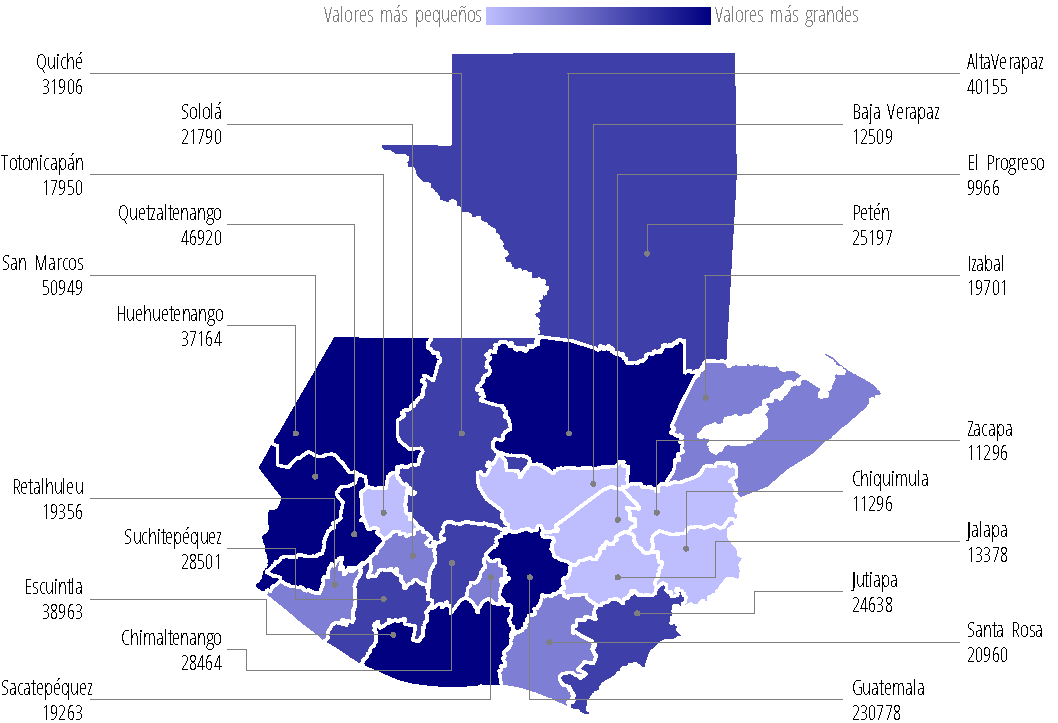
\includegraphics[width=52\cuadri]{C:/Users/INE/Desktop/compendio_educacion/graficas/basicos/1_7.pdf} }{Instituto Nacional de Estadística}




\INEchaptercarta[Indicadores de educación básica]{Indicadores\\ de educación básica}{}


\cajita{Cobertura bruta}{La tasa bruta de cobertura en básico, presentó el año 2009 fue de 66.7\% en el año 2013 fue de 69.3\%, presentando un crecimiento del 4\%.}{Tasa bruta de cobertura del ciclo de educación básica}{República de Guatemala, serie histórica, en porcentaje}{\ \\[0mm]\begin{tikzpicture}[x=1pt,y=1pt]  % Created by tikzDevice version 0.7.0 on 2015-08-28 14:35:24
% !TEX encoding = UTF-8 Unicode
\definecolor[named]{fillColor}{rgb}{1.00,1.00,1.00}
\path[use as bounding box,fill=fillColor,fill opacity=0.00] (0,0) rectangle (289.08,198.74);
\begin{scope}
\path[clip] (  0.00,  0.00) rectangle (289.08,198.74);
\definecolor[named]{drawColor}{rgb}{1.00,1.00,1.00}

\path[draw=drawColor,line width= 0.6pt,line join=round,line cap=round] (  0.00,  0.00) rectangle (289.08,198.74);
\end{scope}
\begin{scope}
\path[clip] (  0.00,  0.00) rectangle (289.08,198.74);

\path[] (  1.64, 17.78) rectangle (280.54,191.48);

\path[] (  1.64, 44.19) --
	(280.54, 44.19);

\path[] (  1.64, 81.22) --
	(280.54, 81.22);

\path[] (  1.64,118.25) --
	(280.54,118.25);

\path[] (  1.64,155.28) --
	(280.54,155.28);

\path[] (  1.64, 25.67) --
	(280.54, 25.67);

\path[] (  1.64, 62.70) --
	(280.54, 62.70);

\path[] (  1.64, 99.73) --
	(280.54, 99.73);

\path[] (  1.64,136.76) --
	(280.54,136.76);

\path[] (  1.64,173.79) --
	(280.54,173.79);

\path[] ( 41.49, 17.78) --
	( 41.49,191.48);

\path[] (107.89, 17.78) --
	(107.89,191.48);

\path[] (174.30, 17.78) --
	(174.30,191.48);

\path[] (240.70, 17.78) --
	(240.70,191.48);
\definecolor[named]{drawColor}{rgb}{0.00,0.00,1.00}

\path[draw=drawColor,line width= 1.7pt,line join=round] ( 41.49,151.95) --
	(107.89,166.39) --
	(174.30,168.98) --
	(240.70,183.59);
\definecolor[named]{drawColor}{rgb}{0.00,0.00,0.00}

\node[text=drawColor,anchor=base,inner sep=0pt, outer sep=0pt, scale=  1.01] at ( 41.49,140.08) {34.1};

\node[text=drawColor,anchor=base east,inner sep=0pt, outer sep=0pt, scale=  1.01] at (104.78,166.39) {38.0};

\node[text=drawColor,anchor=base east,inner sep=0pt, outer sep=0pt, scale=  1.01] at (171.18,168.98) {38.7};

\node[text=drawColor,anchor=base,inner sep=0pt, outer sep=0pt, scale=  1.01] at (240.70,187.54) {42.6};
\definecolor[named]{fillColor}{rgb}{0.00,0.00,0.00}

\path[draw=drawColor,line width= 0.1pt,line join=round,fill=fillColor] (  1.64, 25.67) -- (280.54, 25.67);
\end{scope}
\begin{scope}
\path[clip] (  0.00,  0.00) rectangle (289.08,198.74);

\path[] (  1.64, 17.78) --
	(  1.64,191.48);
\end{scope}
\begin{scope}
\path[clip] (  0.00,  0.00) rectangle (289.08,198.74);

\path[] (  0.00, 25.67) --
	(  1.64, 25.67);

\path[] (  0.00, 62.70) --
	(  1.64, 62.70);

\path[] (  0.00, 99.73) --
	(  1.64, 99.73);

\path[] (  0.00,136.76) --
	(  1.64,136.76);

\path[] (  0.00,173.79) --
	(  1.64,173.79);
\end{scope}
\begin{scope}
\path[clip] (  0.00,  0.00) rectangle (289.08,198.74);

\path[] (  1.64, 17.78) --
	(280.54, 17.78);
\end{scope}
\begin{scope}
\path[clip] (  0.00,  0.00) rectangle (289.08,198.74);

\path[] ( 41.49, 13.51) --
	( 41.49, 17.78);

\path[] (107.89, 13.51) --
	(107.89, 17.78);

\path[] (174.30, 13.51) --
	(174.30, 17.78);

\path[] (240.70, 13.51) --
	(240.70, 17.78);
\end{scope}
\begin{scope}
\path[clip] (  0.00,  0.00) rectangle (289.08,198.74);
\definecolor[named]{drawColor}{rgb}{0.00,0.00,0.00}

\node[text=drawColor,anchor=base,inner sep=0pt, outer sep=0pt, scale=  1.00] at ( 41.49,  2.85) {2010};

\node[text=drawColor,anchor=base,inner sep=0pt, outer sep=0pt, scale=  1.00] at (107.89,  2.85) {2011};

\node[text=drawColor,anchor=base,inner sep=0pt, outer sep=0pt, scale=  1.00] at (174.30,  2.85) {2012};

\node[text=drawColor,anchor=base,inner sep=0pt, outer sep=0pt, scale=  1.00] at (240.70,  2.85) {2013};
\end{scope}
  \end{tikzpicture}}{Instituto Nacional de Estadística}

\cajita{Cobertura bruta por sexo}{La tasa bruta de cobertura en básico por sexo, representa 73.8\% para hombres y 64.8\% para mujeres.}{Tasa bruta de cobertura del ciclo de educación básica, por sexo}{República de Guatemala, año 2013, en porcentaje}{\ \\[0mm]\begin{tikzpicture}[x=1pt,y=1pt]  % Created by tikzDevice version 0.7.0 on 2015-08-28 14:52:30
% !TEX encoding = UTF-8 Unicode
\definecolor[named]{fillColor}{rgb}{1.00,1.00,1.00}
\path[use as bounding box,fill=fillColor,fill opacity=0.00] (0,0) rectangle (289.08,198.74);
\begin{scope}
\path[clip] (  0.00,  0.00) rectangle (289.08,198.74);
\definecolor[named]{drawColor}{rgb}{1.00,1.00,1.00}

\path[draw=drawColor,line width= 0.6pt,line join=round,line cap=round] (  0.00,  0.00) rectangle (289.08,198.74);
\end{scope}
\begin{scope}
\path[clip] (  0.00,  0.00) rectangle (289.08,198.74);

\path[] (  7.11, 20.62) rectangle (289.08,174.77);

\path[] ( 39.65, 20.62) --
	( 39.65,174.77);

\path[] ( 93.87, 20.62) --
	( 93.87,174.77);

\path[] (148.10, 20.62) --
	(148.10,174.77);

\path[] (202.32, 20.62) --
	(202.32,174.77);

\path[] (256.55, 20.62) --
	(256.55,174.77);
\definecolor[named]{drawColor}{rgb}{0.00,0.00,1.00}
\definecolor[named]{fillColor}{rgb}{0.00,0.00,1.00}

\path[draw=drawColor,line width= 0.6pt,line join=round,fill=fillColor] ( 18.64, 20.62) rectangle ( 36.26,172.59);
\definecolor[named]{drawColor}{rgb}{0.62,0.73,1.00}
\definecolor[named]{fillColor}{rgb}{0.62,0.73,1.00}

\path[draw=drawColor,line width= 0.6pt,line join=round,fill=fillColor] ( 43.04, 20.62) rectangle ( 60.66,155.23);
\definecolor[named]{drawColor}{rgb}{0.00,0.00,1.00}
\definecolor[named]{fillColor}{rgb}{0.00,0.00,1.00}

\path[draw=drawColor,line width= 0.6pt,line join=round,fill=fillColor] ( 72.86, 20.62) rectangle ( 90.48,174.77);
\definecolor[named]{drawColor}{rgb}{0.62,0.73,1.00}
\definecolor[named]{fillColor}{rgb}{0.62,0.73,1.00}

\path[draw=drawColor,line width= 0.6pt,line join=round,fill=fillColor] ( 97.26, 20.62) rectangle (114.88,142.20);
\definecolor[named]{drawColor}{rgb}{0.00,0.00,1.00}
\definecolor[named]{fillColor}{rgb}{0.00,0.00,1.00}

\path[draw=drawColor,line width= 0.6pt,line join=round,fill=fillColor] (127.08, 20.62) rectangle (144.71,168.25);
\definecolor[named]{drawColor}{rgb}{0.62,0.73,1.00}
\definecolor[named]{fillColor}{rgb}{0.62,0.73,1.00}

\path[draw=drawColor,line width= 0.6pt,line join=round,fill=fillColor] (151.49, 20.62) rectangle (169.11,144.37);
\definecolor[named]{drawColor}{rgb}{0.00,0.00,1.00}
\definecolor[named]{fillColor}{rgb}{0.00,0.00,1.00}

\path[draw=drawColor,line width= 0.6pt,line join=round,fill=fillColor] (181.31, 20.62) rectangle (198.93,159.57);
\definecolor[named]{drawColor}{rgb}{0.62,0.73,1.00}
\definecolor[named]{fillColor}{rgb}{0.62,0.73,1.00}

\path[draw=drawColor,line width= 0.6pt,line join=round,fill=fillColor] (205.71, 20.62) rectangle (223.33,135.69);
\definecolor[named]{drawColor}{rgb}{0.00,0.00,1.00}
\definecolor[named]{fillColor}{rgb}{0.00,0.00,1.00}

\path[draw=drawColor,line width= 0.6pt,line join=round,fill=fillColor] (235.53, 20.62) rectangle (253.16,133.52);
\definecolor[named]{drawColor}{rgb}{0.62,0.73,1.00}
\definecolor[named]{fillColor}{rgb}{0.62,0.73,1.00}

\path[draw=drawColor,line width= 0.6pt,line join=round,fill=fillColor] (259.93, 20.62) rectangle (277.56,111.81);
\definecolor[named]{drawColor}{rgb}{0.00,0.00,0.00}
\definecolor[named]{fillColor}{rgb}{0.00,0.00,0.00}

\path[draw=drawColor,line width= 0.6pt,line join=round,fill=fillColor] (  7.11, 20.62) -- (289.08, 20.62);

\node[text=drawColor,anchor=base,inner sep=0pt, outer sep=0pt, scale=  0.82] at ( 27.45,175.82) {7.0};

\node[text=drawColor,anchor=base,inner sep=0pt, outer sep=0pt, scale=  0.82] at ( 51.85,158.45) {6.2};

\node[text=drawColor,anchor=base,inner sep=0pt, outer sep=0pt, scale=  0.82] at ( 81.67,177.99) {7.1};

\node[text=drawColor,anchor=base,inner sep=0pt, outer sep=0pt, scale=  0.82] at (106.07,145.42) {5.6};

\node[text=drawColor,anchor=base,inner sep=0pt, outer sep=0pt, scale=  0.82] at (135.90,171.48) {6.8};

\node[text=drawColor,anchor=base,inner sep=0pt, outer sep=0pt, scale=  0.82] at (160.30,147.59) {5.7};

\node[text=drawColor,anchor=base,inner sep=0pt, outer sep=0pt, scale=  0.82] at (190.12,162.79) {6.4};

\node[text=drawColor,anchor=base,inner sep=0pt, outer sep=0pt, scale=  0.82] at (214.52,138.91) {5.3};

\node[text=drawColor,anchor=base,inner sep=0pt, outer sep=0pt, scale=  0.82] at (244.34,136.74) {5.2};

\node[text=drawColor,anchor=base,inner sep=0pt, outer sep=0pt, scale=  0.82] at (268.75,115.03) {4.2};
\end{scope}
\begin{scope}
\path[clip] (  0.00,  0.00) rectangle (289.08,198.74);

\path[] (  7.11, 20.62) --
	(  7.11,174.77);
\end{scope}
\begin{scope}
\path[clip] (  0.00,  0.00) rectangle (289.08,198.74);

\path[] (  7.11, 20.62) --
	(289.08, 20.62);
\end{scope}
\begin{scope}
\path[clip] (  0.00,  0.00) rectangle (289.08,198.74);

\path[] ( 39.65, 16.35) --
	( 39.65, 20.62);

\path[] ( 93.87, 16.35) --
	( 93.87, 20.62);

\path[] (148.10, 16.35) --
	(148.10, 20.62);

\path[] (202.32, 16.35) --
	(202.32, 20.62);

\path[] (256.55, 16.35) --
	(256.55, 20.62);
\end{scope}
\begin{scope}
\path[clip] (  0.00,  0.00) rectangle (289.08,198.74);
\definecolor[named]{drawColor}{rgb}{0.00,0.00,0.00}

\node[text=drawColor,anchor=base,inner sep=0pt, outer sep=0pt, scale=  1.00] at ( 39.65,  5.69) {1987};

\node[text=drawColor,anchor=base,inner sep=0pt, outer sep=0pt, scale=  1.00] at ( 93.87,  5.69) {1995};

\node[text=drawColor,anchor=base,inner sep=0pt, outer sep=0pt, scale=  1.00] at (148.10,  5.69) {1998/99};

\node[text=drawColor,anchor=base,inner sep=0pt, outer sep=0pt, scale=  1.00] at (202.32,  5.69) {2002};

\node[text=drawColor,anchor=base,inner sep=0pt, outer sep=0pt, scale=  1.00] at (256.55,  5.69) {2008/09};
\end{scope}
\coordinate (apoyo) at (50.29,191.13);
\coordinate (longitudFicticia) at (7.11,7.61);
\coordinate (longitud) at (7.11,7.11);
\coordinate (desX) at (142.09,0);
\coordinate (desY) at (0,0.25);
\definecolor[named]{ct1}{HTML}{
0000FF
}
\definecolor[named]{ct2}{HTML}{
9DBBFF
}
\definecolor[named]{ctb1}{HTML}{
0000FF
}
\definecolor[named]{ctb2}{HTML}{
9DBBFF
}
\path [fill=none] (apoyo) rectangle ($(apoyo)+(longitudFicticia)$)
node [xshift=0.3cm,inner sep=0pt, outer sep=0pt,midway,right,scale = 0.9]{Observados};
\draw [color = ctb1,fill=ct1] ( $(apoyo)  + (desY) $) rectangle ($(apoyo)+ (desY) +(longitud)$);
\path [fill=none] ($(apoyo)+(desX)$) rectangle ($(apoyo)+(desX)+(longitudFicticia)$)
node [xshift=0.3cm,inner sep=0pt, outer sep=0pt,midway,right,scale = 0.9]{Deseados};
\draw [color = ctb2 ,fill=ct2] ( $(apoyo)  + (desY) + (desX) $) rectangle ($(apoyo)+ (desY)+ (desX) +(longitud)$);
  \end{tikzpicture}}{Instituto Nacional de Estadística}

\cajota{Cobertura bruta en los departamentos}{En el siguiente mapa se observan los departamentos donde hubo baja tasa bruta de cobertura en básico fueron: Huehuetenango  40.5\%, Quiché 40.7\% y Alta Verapaz 42.1\%.\\  
	
	Los departamentos donde hubo alta tasa bruta de cobertura en básico: Retalhuleu 86.6\%, El Progreso 86.9\% y Guatemala 111.9\%.}{Tasa bruta de cobertura del ciclo de educación básica}{Por departamento, año 2013, en porcentaje}{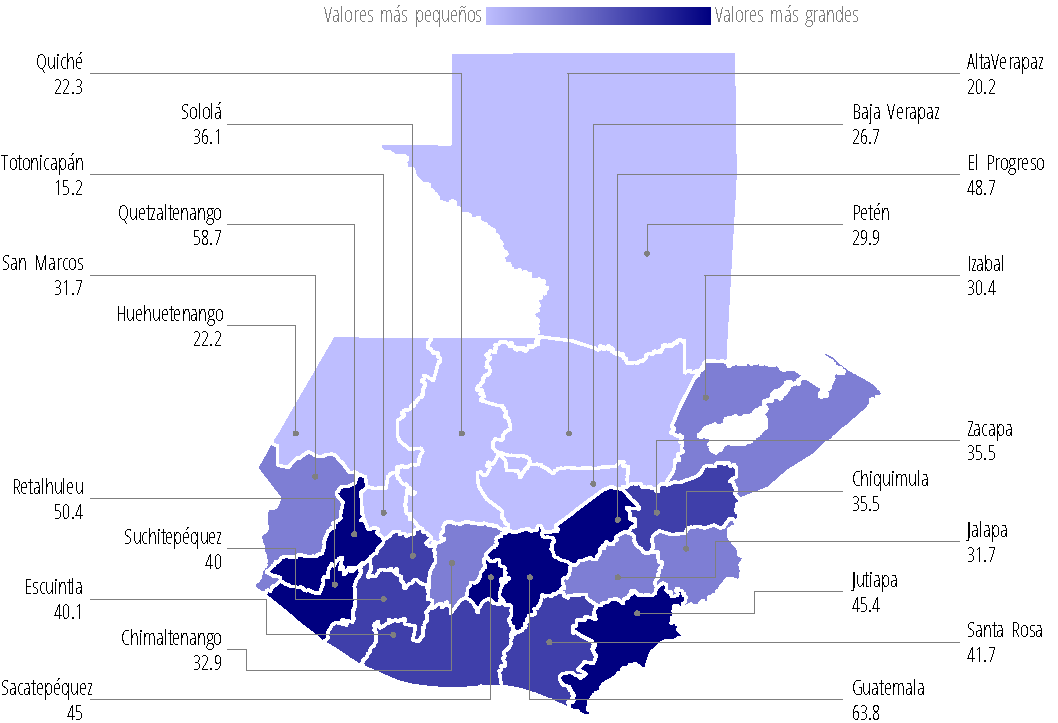
\includegraphics[width=52\cuadri]{C:/Users/INE/Desktop/compendio_educacion/graficas/basicos/1_10.pdf}}{Instituto Nacional de Estadística}

\cajita{Cobertura neta}{La tasa neta de cobertura en básico, presentó en el año 2009 el 40.3\% y en el año 2013 fue de 44\%, presentando un crecimiento de 9.4\%.}{Tasa neta de cobertura del ciclo de educación básica}{República de Guatemala, serie histórica, en porcentaje}{\ \\[0mm]\begin{tikzpicture}[x=1pt,y=1pt]  % Created by tikzDevice version 0.7.0 on 2015-08-31 18:32:55
% !TEX encoding = UTF-8 Unicode
\definecolor[named]{fillColor}{rgb}{1.00,1.00,1.00}
\path[use as bounding box,fill=fillColor,fill opacity=0.00] (0,0) rectangle (289.08,198.74);
\begin{scope}
\path[clip] (  0.00,  0.00) rectangle (289.08,198.74);
\definecolor[named]{drawColor}{rgb}{1.00,1.00,1.00}

\path[draw=drawColor,line width= 0.6pt,line join=round,line cap=round] (  0.00,  0.00) rectangle (289.08,198.74);
\end{scope}
\begin{scope}
\path[clip] (  0.00,  0.00) rectangle (289.08,198.74);

\path[] (  1.64, 17.78) rectangle (280.54,191.48);

\path[] (  1.64, 52.90) --
	(280.54, 52.90);

\path[] (  1.64,107.35) --
	(280.54,107.35);

\path[] (  1.64,161.81) --
	(280.54,161.81);

\path[] (  1.64, 25.67) --
	(280.54, 25.67);

\path[] (  1.64, 80.12) --
	(280.54, 80.12);

\path[] (  1.64,134.58) --
	(280.54,134.58);

\path[] (  1.64,189.03) --
	(280.54,189.03);

\path[] ( 33.83, 17.78) --
	( 33.83,191.48);

\path[] ( 87.46, 17.78) --
	( 87.46,191.48);

\path[] (141.09, 17.78) --
	(141.09,191.48);

\path[] (194.73, 17.78) --
	(194.73,191.48);

\path[] (248.36, 17.78) --
	(248.36,191.48);
\definecolor[named]{drawColor}{rgb}{0.00,0.00,1.00}

\path[draw=drawColor,line width= 1.7pt,line join=round] ( 33.83,147.65) --
	( 87.46,159.63) --
	(141.09,172.70) --
	(194.73,180.32) --
	(248.36,183.59);
\definecolor[named]{drawColor}{rgb}{0.00,0.00,0.00}

\node[text=drawColor,anchor=base,inner sep=0pt, outer sep=0pt, scale=  1.01] at ( 33.83,135.78) {21.2};

\node[text=drawColor,anchor=base east,inner sep=0pt, outer sep=0pt, scale=  1.01] at ( 84.34,159.63) {22.3};

\node[text=drawColor,anchor=base east,inner sep=0pt, outer sep=0pt, scale=  1.01] at (137.98,172.70) {23.5};

\node[text=drawColor,anchor=base east,inner sep=0pt, outer sep=0pt, scale=  1.01] at (191.61,180.32) {24.2};

\node[text=drawColor,anchor=base,inner sep=0pt, outer sep=0pt, scale=  1.01] at (248.36,187.54) {24.5};
\definecolor[named]{fillColor}{rgb}{0.00,0.00,0.00}

\path[draw=drawColor,line width= 0.1pt,line join=round,fill=fillColor] (  1.64, 25.67) -- (280.54, 25.67);
\end{scope}
\begin{scope}
\path[clip] (  0.00,  0.00) rectangle (289.08,198.74);

\path[] (  1.64, 17.78) --
	(  1.64,191.48);
\end{scope}
\begin{scope}
\path[clip] (  0.00,  0.00) rectangle (289.08,198.74);

\path[] (  0.00, 25.67) --
	(  1.64, 25.67);

\path[] (  0.00, 80.12) --
	(  1.64, 80.12);

\path[] (  0.00,134.58) --
	(  1.64,134.58);

\path[] (  0.00,189.03) --
	(  1.64,189.03);
\end{scope}
\begin{scope}
\path[clip] (  0.00,  0.00) rectangle (289.08,198.74);

\path[] (  1.64, 17.78) --
	(280.54, 17.78);
\end{scope}
\begin{scope}
\path[clip] (  0.00,  0.00) rectangle (289.08,198.74);

\path[] ( 33.83, 13.51) --
	( 33.83, 17.78);

\path[] ( 87.46, 13.51) --
	( 87.46, 17.78);

\path[] (141.09, 13.51) --
	(141.09, 17.78);

\path[] (194.73, 13.51) --
	(194.73, 17.78);

\path[] (248.36, 13.51) --
	(248.36, 17.78);
\end{scope}
\begin{scope}
\path[clip] (  0.00,  0.00) rectangle (289.08,198.74);
\definecolor[named]{drawColor}{rgb}{0.00,0.00,0.00}

\node[text=drawColor,anchor=base,inner sep=0pt, outer sep=0pt, scale=  1.00] at ( 33.83,  2.85) {2009};

\node[text=drawColor,anchor=base,inner sep=0pt, outer sep=0pt, scale=  1.00] at ( 87.46,  2.85) {2010};

\node[text=drawColor,anchor=base,inner sep=0pt, outer sep=0pt, scale=  1.00] at (141.09,  2.85) {2011};

\node[text=drawColor,anchor=base,inner sep=0pt, outer sep=0pt, scale=  1.00] at (194.73,  2.85) {2012};

\node[text=drawColor,anchor=base,inner sep=0pt, outer sep=0pt, scale=  1.00] at (248.36,  2.85) {2013};
\end{scope}
  \end{tikzpicture}}{Instituto Nacional de Estadística}

\cajita{Cobertura neta por sexo}{La tasa neta de cobertura en básico por sexo, representa el 45.6\% para hombres y 42.5\% para las mujeres.}{Tasa neta de cobertura del ciclo de educación básica, por sexo}{República de Guatemala, año 2013, en porcentaje}{\ \\[0mm]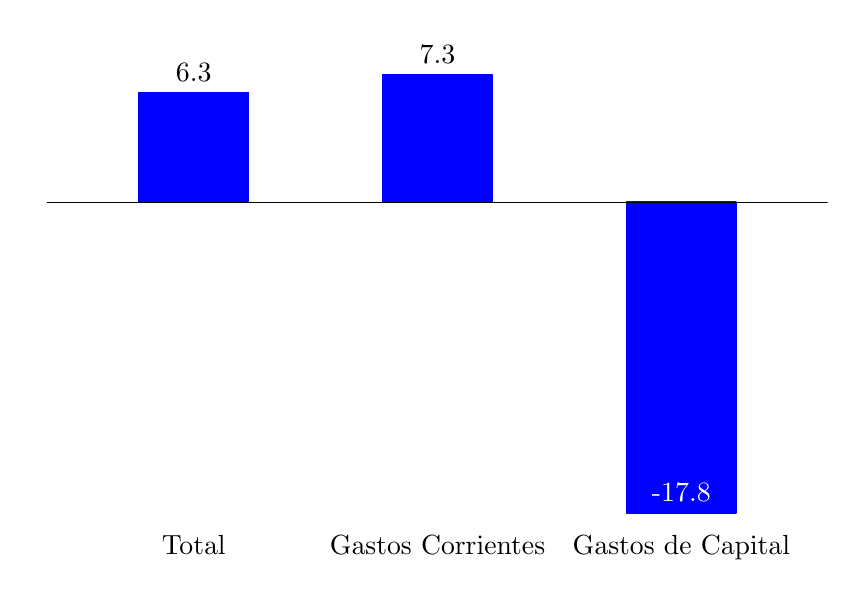
\begin{tikzpicture}[x=1pt,y=1pt]  % Created by tikzDevice version 0.7.0 on 2015-09-08 19:17:12
% !TEX encoding = UTF-8 Unicode
\definecolor[named]{fillColor}{rgb}{1.00,1.00,1.00}
\path[use as bounding box,fill=fillColor,fill opacity=0.00] (0,0) rectangle (289.08,198.74);
\begin{scope}
\path[clip] (  0.00,  0.00) rectangle (289.08,198.74);
\definecolor[named]{drawColor}{rgb}{1.00,1.00,1.00}

\path[draw=drawColor,line width= 0.6pt,line join=round,line cap=round] (  0.00,  0.00) rectangle (289.08,198.74);
\end{scope}
\begin{scope}
\path[clip] (  0.00,  0.00) rectangle (289.08,198.74);

\path[] (  7.11, 23.47) rectangle (289.08,181.67);

\path[] ( 59.98, 23.47) --
	( 59.98,181.67);

\path[] (148.10, 23.47) --
	(148.10,181.67);

\path[] (236.21, 23.47) --
	(236.21,181.67);
\definecolor[named]{drawColor}{rgb}{0.00,0.00,1.00}
\definecolor[named]{fillColor}{rgb}{0.00,0.00,1.00}

\path[draw=drawColor,line width= 0.6pt,line join=round,fill=fillColor] ( 40.16,135.66) rectangle ( 79.81,175.37);

\path[draw=drawColor,line width= 0.6pt,line join=round,fill=fillColor] (128.27,135.66) rectangle (167.92,181.67);

\path[draw=drawColor,line width= 0.6pt,line join=round,fill=fillColor] (216.39, 23.47) rectangle (256.04,135.66);
\definecolor[named]{drawColor}{rgb}{0.00,0.00,0.00}
\definecolor[named]{fillColor}{rgb}{0.00,0.00,0.00}

\path[draw=drawColor,line width= 0.1pt,line join=round,fill=fillColor] (  7.11,135.66) -- (289.08,135.66);

\node[text=drawColor,anchor=base,inner sep=0pt, outer sep=0pt, scale=  1.01] at ( 59.98,179.32) {6.3};

\node[text=drawColor,anchor=base,inner sep=0pt, outer sep=0pt, scale=  1.01] at (148.10,185.63) {7.3};

\node[text=white,anchor=base,inner sep=0pt, outer sep=0pt, scale=  1.01] at (236.21, 27.42) {-17.8};
\end{scope}
\begin{scope}
\path[clip] (  0.00,  0.00) rectangle (289.08,198.74);

\path[] (  7.11, 23.47) --
	(  7.11,181.67);
\end{scope}
\begin{scope}
\path[clip] (  0.00,  0.00) rectangle (289.08,198.74);

\path[] (  7.11, 23.47) --
	(289.08, 23.47);
\end{scope}
\begin{scope}
\path[clip] (  0.00,  0.00) rectangle (289.08,198.74);

\path[] ( 59.98, 19.20) --
	( 59.98, 23.47);

\path[] (148.10, 19.20) --
	(148.10, 23.47);

\path[] (236.21, 19.20) --
	(236.21, 23.47);
\end{scope}
\begin{scope}
\path[clip] (  0.00,  0.00) rectangle (289.08,198.74);
\definecolor[named]{drawColor}{rgb}{0.00,0.00,0.00}

\node[text=drawColor,anchor=base,inner sep=0pt, outer sep=0pt, scale=  1.00] at ( 59.98,  8.54) {Total};

\node[text=drawColor,anchor=base,inner sep=0pt, outer sep=0pt, scale=  1.00] at (148.10,  8.54) {Gastos Corrientes};

\node[text=drawColor,anchor=base,inner sep=0pt, outer sep=0pt, scale=  1.00] at (236.21,  8.54) {Gastos de Capital};
\end{scope}
  \end{tikzpicture}}{Instituto Nacional de Estadística}

\cajota{Cobertura neta en los departamentos}{En el siguiente mapa se observan los departamentos donde hubo menor tasa neta de cobertura en básico, fueron los siguientes: Alta Verapaz 22.6\%,  Quiché 24.7\% y Huehuetenango 25.7\%.\\ 
	
	 Los departamentos donde hubo alta tasa neta de cobertura en básico fueron: Sacatepéquez 57.7\%, El Progreso 58\% y Guatemala 69.4\%. }{Tasa neta de cobertura del ciclo de educación básica}{Por departamento, año 2013, en porcentaje}{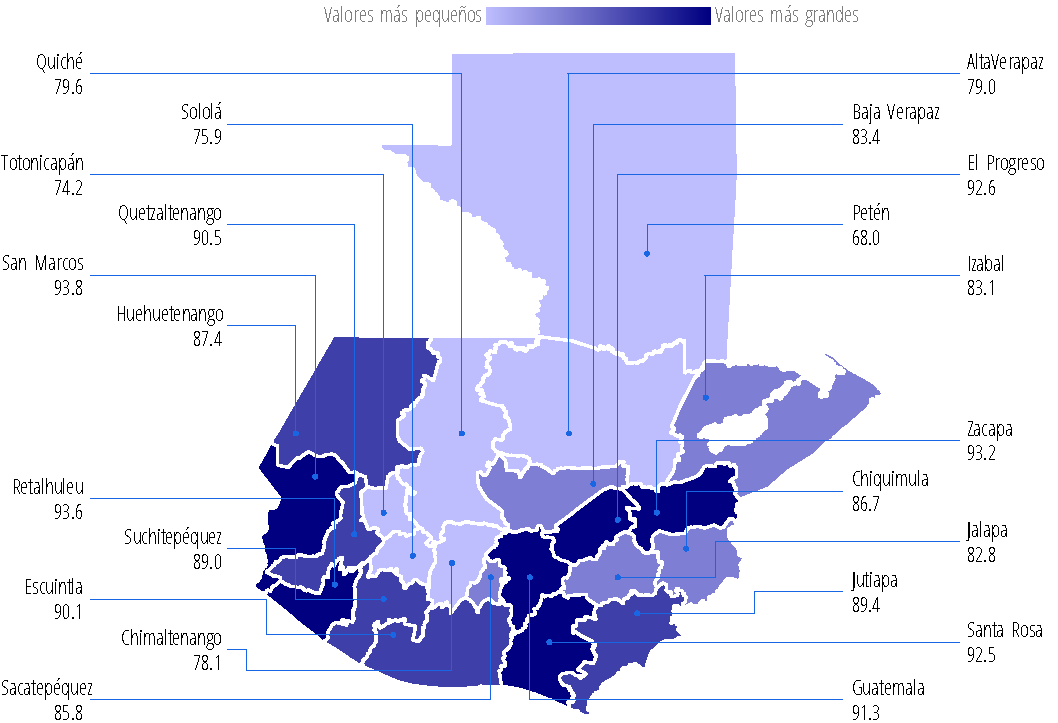
\includegraphics[width=52\cuadri]{C:/Users/INE/Desktop/compendio_educacion/graficas/basicos/1_13.pdf}}{Instituto Nacional de Estadística}




\cajita{Repitencia}{La tasa de repitencia en básico, presentó el año 2009 el 3.1\% y en el año 2013 fue de 4.5\%, presentando un crecimiento del 48.4\%.}{Tasa de repitencia del ciclo de educación básica}{República de Guatemala, serie histórica, en porcentaje}{\ \\[0mm]\begin{tikzpicture}[x=1pt,y=1pt]  % Created by tikzDevice version 0.7.0 on 2015-08-31 18:26:28
% !TEX encoding = UTF-8 Unicode
\definecolor[named]{fillColor}{rgb}{1.00,1.00,1.00}
\path[use as bounding box,fill=fillColor,fill opacity=0.00] (0,0) rectangle (289.08,198.74);
\begin{scope}
\path[clip] (  0.00,  0.00) rectangle (289.08,198.74);
\definecolor[named]{drawColor}{rgb}{1.00,1.00,1.00}

\path[draw=drawColor,line width= 0.6pt,line join=round,line cap=round] (  0.00,  0.00) rectangle (289.08,198.74);
\end{scope}
\begin{scope}
\path[clip] (  0.00,  0.00) rectangle (289.08,198.74);

\path[] ( -2.73, 17.78) rectangle (280.54,191.48);

\path[] (  0.00, 53.87) --
	(280.54, 53.87);

\path[] (  0.00,110.27) --
	(280.54,110.27);

\path[] (  0.00,166.67) --
	(280.54,166.67);

\path[] (  0.00, 25.67) --
	(280.54, 25.67);

\path[] (  0.00, 82.07) --
	(280.54, 82.07);

\path[] (  0.00,138.47) --
	(280.54,138.47);

\path[] ( 29.95, 17.78) --
	( 29.95,191.48);

\path[] ( 84.43, 17.78) --
	( 84.43,191.48);

\path[] (138.90, 17.78) --
	(138.90,191.48);

\path[] (193.38, 17.78) --
	(193.38,191.48);

\path[] (247.86, 17.78) --
	(247.86,191.48);
\definecolor[named]{drawColor}{rgb}{0.00,0.00,1.00}

\path[draw=drawColor,line width= 1.7pt,line join=round] ( 29.95,113.09) --
	( 84.43,110.27) --
	(138.90,104.63) --
	(193.38,183.59) --
	(247.86,152.57);
\definecolor[named]{drawColor}{rgb}{0.00,0.00,0.00}

\node[text=drawColor,anchor=base,inner sep=0pt, outer sep=0pt, scale=  1.01] at ( 29.95,117.05) {3.1};

\node[text=drawColor,anchor=base west,inner sep=0pt, outer sep=0pt, scale=  1.01] at ( 84.43,114.23) {3.0};

\node[text=drawColor,anchor=base,inner sep=0pt, outer sep=0pt, scale=  1.01] at (138.90, 92.76) {2.8};

\node[text=drawColor,anchor=base,inner sep=0pt, outer sep=0pt, scale=  1.01] at (193.38,187.54) {5.6};

\node[text=drawColor,anchor=base,inner sep=0pt, outer sep=0pt, scale=  1.01] at (247.86,140.70) {4.5};
\definecolor[named]{fillColor}{rgb}{0.00,0.00,0.00}

\path[draw=drawColor,line width= 0.1pt,line join=round,fill=fillColor] (  0.00, 25.67) -- (280.54, 25.67);
\end{scope}
\begin{scope}
\path[clip] (  0.00,  0.00) rectangle (289.08,198.74);

\path[] (  0.00, 17.78) --
	(280.54, 17.78);
\end{scope}
\begin{scope}
\path[clip] (  0.00,  0.00) rectangle (289.08,198.74);

\path[] ( 29.95, 13.51) --
	( 29.95, 17.78);

\path[] ( 84.43, 13.51) --
	( 84.43, 17.78);

\path[] (138.90, 13.51) --
	(138.90, 17.78);

\path[] (193.38, 13.51) --
	(193.38, 17.78);

\path[] (247.86, 13.51) --
	(247.86, 17.78);
\end{scope}
\begin{scope}
\path[clip] (  0.00,  0.00) rectangle (289.08,198.74);
\definecolor[named]{drawColor}{rgb}{0.00,0.00,0.00}

\node[text=drawColor,anchor=base,inner sep=0pt, outer sep=0pt, scale=  1.00] at ( 29.95,  2.85) {2009};

\node[text=drawColor,anchor=base,inner sep=0pt, outer sep=0pt, scale=  1.00] at ( 84.43,  2.85) {2010};

\node[text=drawColor,anchor=base,inner sep=0pt, outer sep=0pt, scale=  1.00] at (138.90,  2.85) {2011};

\node[text=drawColor,anchor=base,inner sep=0pt, outer sep=0pt, scale=  1.00] at (193.38,  2.85) {2012};

\node[text=drawColor,anchor=base,inner sep=0pt, outer sep=0pt, scale=  1.00] at (247.86,  2.85) {2013};
\end{scope}
  \end{tikzpicture}}{Instituto Nacional de Estadística}

\cajita{Repitencia por sexo}{La tasa de repitencia en básico por sexo, representa el 5.5\% para hombres y 3.5\% para las mujeres.}{Tasa de repitencia del ciclo de educación básica, por sexo}{República de Guatemala, año 2013, en porcentaje}{\ \\[0mm]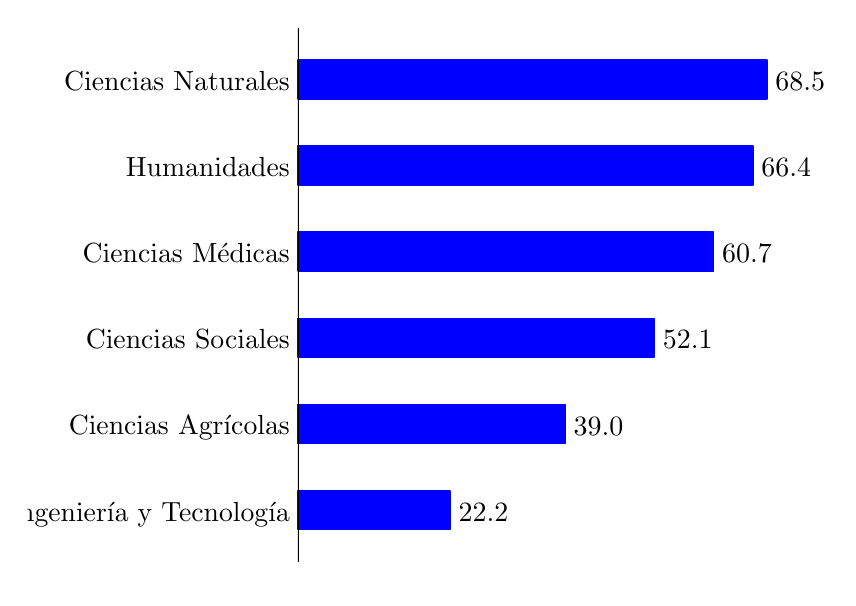
\begin{tikzpicture}[x=1pt,y=1pt]  % Created by tikzDevice version 0.7.0 on 2015-08-31 14:52:10
% !TEX encoding = UTF-8 Unicode
\definecolor[named]{fillColor}{rgb}{1.00,1.00,1.00}
\path[use as bounding box,fill=fillColor,fill opacity=0.00] (0,0) rectangle (289.08,198.74);
\begin{scope}
\path[clip] (  0.00,  0.00) rectangle (289.08,198.74);
\definecolor[named]{drawColor}{rgb}{1.00,1.00,1.00}

\path[draw=drawColor,line width= 0.6pt,line join=round,line cap=round] (  0.00,  0.00) rectangle (289.08,198.74);
\end{scope}
\begin{scope}
\path[clip] (  0.00,  0.00) rectangle (289.08,198.74);

\path[] ( 97.57,  5.69) rectangle (267.09,198.74);

\path[] ( 97.57, 24.37) --
	(267.09, 24.37);

\path[] ( 97.57, 55.51) --
	(267.09, 55.51);

\path[] ( 97.57, 86.65) --
	(267.09, 86.65);

\path[] ( 97.57,117.79) --
	(267.09,117.79);

\path[] ( 97.57,148.92) --
	(267.09,148.92);

\path[] ( 97.57,180.06) --
	(267.09,180.06);
\definecolor[named]{drawColor}{rgb}{0.00,0.00,1.00}
\definecolor[named]{fillColor}{rgb}{0.00,0.00,1.00}

\path[draw=drawColor,line width= 0.6pt,line join=round,fill=fillColor] ( 97.57, 17.37) rectangle (152.65, 31.38);

\path[draw=drawColor,line width= 0.6pt,line join=round,fill=fillColor] ( 97.57, 48.50) rectangle (194.18, 62.52);

\path[draw=drawColor,line width= 0.6pt,line join=round,fill=fillColor] ( 97.57, 79.64) rectangle (226.45, 93.65);

\path[draw=drawColor,line width= 0.6pt,line join=round,fill=fillColor] ( 97.57,110.78) rectangle (247.82,124.79);

\path[draw=drawColor,line width= 0.6pt,line join=round,fill=fillColor] ( 97.57,141.92) rectangle (262.01,155.93);

\path[draw=drawColor,line width= 0.6pt,line join=round,fill=fillColor] ( 97.57,173.05) rectangle (267.09,187.07);
\definecolor[named]{drawColor}{rgb}{0.00,0.00,0.00}
\definecolor[named]{fillColor}{rgb}{0.00,0.00,0.00}

\path[draw=drawColor,line width= 0.1pt,line join=round,fill=fillColor] ( 97.57,  5.69) -- ( 97.57,198.74);

\node[text=drawColor,anchor=base west,inner sep=0pt, outer sep=0pt, scale=  1.01] at (155.76, 20.42) {22.2};

\node[text=drawColor,anchor=base west,inner sep=0pt, outer sep=0pt, scale=  1.01] at (197.29, 51.55) {39.0};

\node[text=drawColor,anchor=base west,inner sep=0pt, outer sep=0pt, scale=  1.01] at (229.57, 82.69) {52.1};

\node[text=drawColor,anchor=base west,inner sep=0pt, outer sep=0pt, scale=  1.01] at (250.94,113.83) {60.7};

\node[text=drawColor,anchor=base west,inner sep=0pt, outer sep=0pt, scale=  1.01] at (265.12,144.97) {66.4};

\node[text=drawColor,anchor=base west,inner sep=0pt, outer sep=0pt, scale=  1.01] at (270.20,176.10) {68.5};
\end{scope}
\begin{scope}
\path[clip] (  0.00,  0.00) rectangle (289.08,198.74);

\path[] ( 97.57,  5.69) --
	( 97.57,198.74);
\end{scope}
\begin{scope}
\path[clip] (  0.00,  0.00) rectangle (289.08,198.74);
\definecolor[named]{drawColor}{rgb}{0.00,0.00,0.00}

\node[text=drawColor,anchor=base east,inner sep=0pt, outer sep=0pt, scale=  1.00] at ( 94.72, 20.46) {Ingenier\'ia y Tecnolog\'ia};

\node[text=drawColor,anchor=base east,inner sep=0pt, outer sep=0pt, scale=  1.00] at ( 94.72, 51.60) {Ciencias Agr\'icolas};

\node[text=drawColor,anchor=base east,inner sep=0pt, outer sep=0pt, scale=  1.00] at ( 94.72, 82.74) {Ciencias Sociales};

\node[text=drawColor,anchor=base east,inner sep=0pt, outer sep=0pt, scale=  1.00] at ( 94.72,113.88) {Ciencias M\'edicas};

\node[text=drawColor,anchor=base east,inner sep=0pt, outer sep=0pt, scale=  1.00] at ( 94.72,145.01) {Humanidades};

\node[text=drawColor,anchor=base east,inner sep=0pt, outer sep=0pt, scale=  1.00] at ( 94.72,176.15) {Ciencias Naturales };
\end{scope}
\begin{scope}
\path[clip] (  0.00,  0.00) rectangle (289.08,198.74);

\path[] ( 94.72, 24.37) --
	( 98.99, 24.37);

\path[] ( 94.72, 55.51) --
	( 98.99, 55.51);

\path[] ( 94.72, 86.65) --
	( 98.99, 86.65);

\path[] ( 94.72,117.79) --
	( 98.99,117.79);

\path[] ( 94.72,148.92) --
	( 98.99,148.92);

\path[] ( 94.72,180.06) --
	( 98.99,180.06);
\end{scope}
\begin{scope}
\path[clip] (  0.00,  0.00) rectangle (289.08,198.74);

\path[] ( 97.57,  5.69) --
	(267.09,  5.69);
\end{scope}
  \end{tikzpicture}}{Instituto Nacional de Estadística}

\cajota{Repitencia en los departamentos}{En el siguiente mapa se observan los departamentos donde hubo baja tasa de repitencia en básico fueron: Petén 2.3\%, Jutiapa 2.4\% y Retalhuleu 2.4\%.\\ 
	
	 Los departamentos donde hubo alta tasa de repitencia en básico: Totonicapán 6.3\%, Chimaltenango 6.8\% y Sacatepéquez 8.5\%. El departamento de Guatemala presentó una tasa de repitencia de 5\%.}{Tasa de repitencia del ciclo de educación básica}{Por departamento, año 2013, en porcentaje}{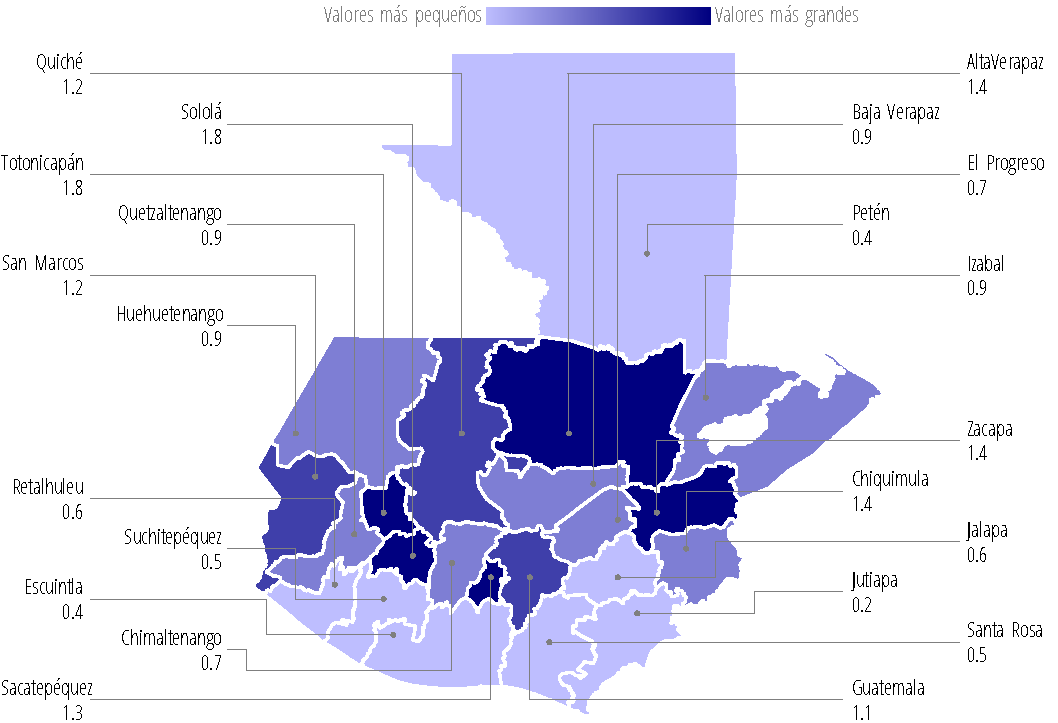
\includegraphics[width=52\cuadri]{C:/Users/INE/Desktop/compendio_educacion/graficas/basicos/1_16.pdf}}{Instituto Nacional de Estadística}






\cajita{Sobre-edad}{La tasa de sobre-edad en básico, presentó el año 2009 el 34\% y en el año 2013 fue de 28.2\%, presentando un decrecimiento de 17.3\%.}{Tasa de sobre-edad del ciclo de educación básica}{República de Guatemala, serie histórica, en porcentaje}{\ \\[0mm]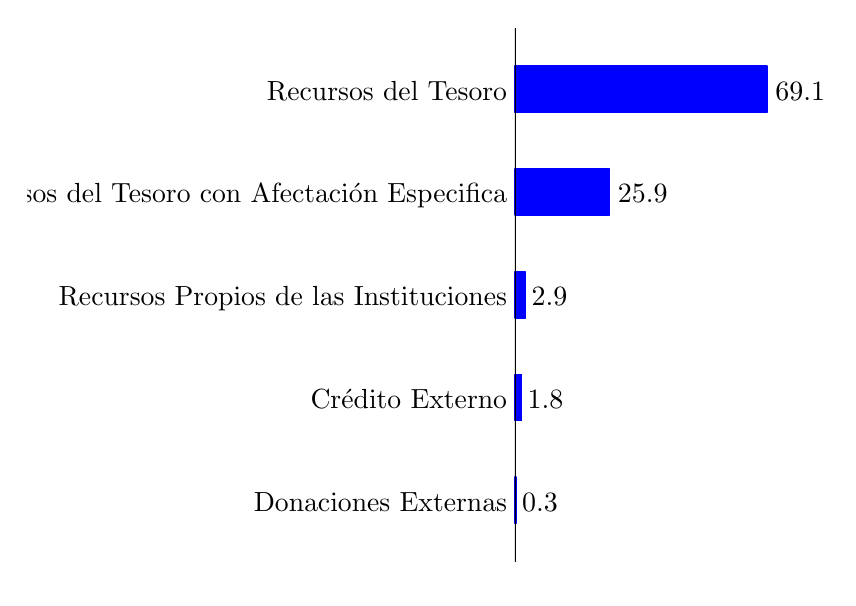
\begin{tikzpicture}[x=1pt,y=1pt]  % Created by tikzDevice version 0.7.0 on 2015-08-28 16:35:08
% !TEX encoding = UTF-8 Unicode
\definecolor[named]{fillColor}{rgb}{1.00,1.00,1.00}
\path[use as bounding box,fill=fillColor,fill opacity=0.00] (0,0) rectangle (289.08,198.74);
\begin{scope}
\path[clip] (  0.00,  0.00) rectangle (289.08,198.74);
\definecolor[named]{drawColor}{rgb}{1.00,1.00,1.00}

\path[draw=drawColor,line width= 0.6pt,line join=round,line cap=round] (  0.00,  0.00) rectangle (289.08,198.74);
\end{scope}
\begin{scope}
\path[clip] (  0.00,  0.00) rectangle (289.08,198.74);

\path[] (176.08,  5.69) rectangle (267.09,198.74);

\path[] (176.08, 27.97) --
	(267.09, 27.97);

\path[] (176.08, 65.09) --
	(267.09, 65.09);

\path[] (176.08,102.22) --
	(267.09,102.22);

\path[] (176.08,139.34) --
	(267.09,139.34);

\path[] (176.08,176.47) --
	(267.09,176.47);
\definecolor[named]{drawColor}{rgb}{0.00,0.00,1.00}
\definecolor[named]{fillColor}{rgb}{0.00,0.00,1.00}

\path[draw=drawColor,line width= 0.6pt,line join=round,fill=fillColor] (176.08, 19.61) rectangle (176.47, 36.32);

\path[draw=drawColor,line width= 0.6pt,line join=round,fill=fillColor] (176.08, 56.74) rectangle (178.45, 73.44);

\path[draw=drawColor,line width= 0.6pt,line join=round,fill=fillColor] (176.08, 93.86) rectangle (179.90,110.57);

\path[draw=drawColor,line width= 0.6pt,line join=round,fill=fillColor] (176.08,130.99) rectangle (210.19,147.70);

\path[draw=drawColor,line width= 0.6pt,line join=round,fill=fillColor] (176.08,168.11) rectangle (267.09,184.82);
\definecolor[named]{drawColor}{rgb}{0.00,0.00,0.00}
\definecolor[named]{fillColor}{rgb}{0.00,0.00,0.00}

\path[draw=drawColor,line width= 0.1pt,line join=round,fill=fillColor] (176.08,  5.69) -- (176.08,198.74);

\node[text=drawColor,anchor=base west,inner sep=0pt, outer sep=0pt, scale=  1.01] at (178.70, 24.01) {0.3};

\node[text=drawColor,anchor=base west,inner sep=0pt, outer sep=0pt, scale=  1.01] at (180.68, 61.13) {1.8};

\node[text=drawColor,anchor=base west,inner sep=0pt, outer sep=0pt, scale=  1.01] at (182.13, 98.26) {2.9};

\node[text=drawColor,anchor=base west,inner sep=0pt, outer sep=0pt, scale=  1.01] at (213.30,135.39) {25.9};

\node[text=drawColor,anchor=base west,inner sep=0pt, outer sep=0pt, scale=  1.01] at (270.20,172.51) {69.1};
\end{scope}
\begin{scope}
\path[clip] (  0.00,  0.00) rectangle (289.08,198.74);

\path[] (176.08,  5.69) --
	(176.08,198.74);
\end{scope}
\begin{scope}
\path[clip] (  0.00,  0.00) rectangle (289.08,198.74);
\definecolor[named]{drawColor}{rgb}{0.00,0.00,0.00}

\node[text=drawColor,anchor=base east,inner sep=0pt, outer sep=0pt, scale=  1.00] at (173.23, 24.06) {Donaciones Externas};

\node[text=drawColor,anchor=base east,inner sep=0pt, outer sep=0pt, scale=  1.00] at (173.23, 61.18) {Cr\'edito Externo};

\node[text=drawColor,anchor=base east,inner sep=0pt, outer sep=0pt, scale=  1.00] at (173.23, 98.31) {Recursos Propios de las Instituciones};

\node[text=drawColor,anchor=base east,inner sep=0pt, outer sep=0pt, scale=  1.00] at (173.23,135.43) {Recursos del Tesoro con Afectaci\'on Especifica};

\node[text=drawColor,anchor=base east,inner sep=0pt, outer sep=0pt, scale=  1.00] at (173.23,172.56) {Recursos del Tesoro};
\end{scope}
\begin{scope}
\path[clip] (  0.00,  0.00) rectangle (289.08,198.74);

\path[] (173.23, 27.97) --
	(177.50, 27.97);

\path[] (173.23, 65.09) --
	(177.50, 65.09);

\path[] (173.23,102.22) --
	(177.50,102.22);

\path[] (173.23,139.34) --
	(177.50,139.34);

\path[] (173.23,176.47) --
	(177.50,176.47);
\end{scope}
\begin{scope}
\path[clip] (  0.00,  0.00) rectangle (289.08,198.74);

\path[] (176.08,  5.69) --
	(267.09,  5.69);
\end{scope}
  \end{tikzpicture}}{Instituto Nacional de Estadística}

\cajita{Sobre-edad por sexo}{La tasa de sobre-edad en básico por sexo, representa el 31.4\% para hombres y 24.4\% para las mujeres.}{Tasa de sobre-edad del ciclo de educación básica, por sexo}{República de Guatemala, año 2013, en porcentaje}{\ \\[0mm]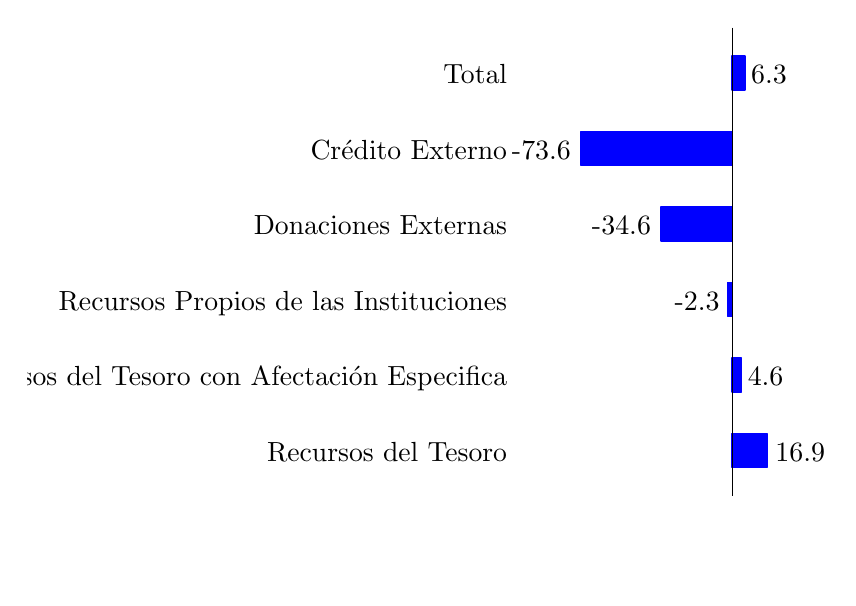
\begin{tikzpicture}[x=1pt,y=1pt]  % Created by tikzDevice version 0.7.0 on 2015-08-28 16:35:09
% !TEX encoding = UTF-8 Unicode
\definecolor[named]{fillColor}{rgb}{1.00,1.00,1.00}
\path[use as bounding box,fill=fillColor,fill opacity=0.00] (0,0) rectangle (289.08,198.74);
\begin{scope}
\path[clip] (  0.00,  0.00) rectangle (289.08,198.74);
\definecolor[named]{drawColor}{rgb}{1.00,1.00,1.00}

\path[draw=drawColor,line width= 0.6pt,line join=round,line cap=round] (  0.00,  0.00) rectangle (289.08,198.74);
\end{scope}
\begin{scope}
\path[clip] (  0.00,  0.00) rectangle (289.08,198.74);

\path[] (199.99, 29.60) rectangle (267.09,198.74);

\path[] (199.99, 45.97) --
	(267.09, 45.97);

\path[] (199.99, 73.25) --
	(267.09, 73.25);

\path[] (199.99,100.53) --
	(267.09,100.53);

\path[] (199.99,127.81) --
	(267.09,127.81);

\path[] (199.99,155.09) --
	(267.09,155.09);

\path[] (199.99,182.37) --
	(267.09,182.37);
\definecolor[named]{drawColor}{rgb}{0.00,0.00,1.00}
\definecolor[named]{fillColor}{rgb}{0.00,0.00,1.00}

\path[draw=drawColor,line width= 0.6pt,line join=round,fill=fillColor] (254.56, 39.83) rectangle (267.09, 52.11);

\path[draw=drawColor,line width= 0.6pt,line join=round,fill=fillColor] (254.56, 67.11) rectangle (257.97, 79.39);

\path[draw=drawColor,line width= 0.6pt,line join=round,fill=fillColor] (252.85, 94.39) rectangle (254.56,106.67);

\path[draw=drawColor,line width= 0.6pt,line join=round,fill=fillColor] (228.90,121.67) rectangle (254.56,133.95);

\path[draw=drawColor,line width= 0.6pt,line join=round,fill=fillColor] (199.99,148.95) rectangle (254.56,161.23);

\path[draw=drawColor,line width= 0.6pt,line join=round,fill=fillColor] (254.56,176.24) rectangle (259.23,188.51);
\definecolor[named]{drawColor}{rgb}{0.00,0.00,0.00}
\definecolor[named]{fillColor}{rgb}{0.00,0.00,0.00}

\path[draw=drawColor,line width= 0.1pt,line join=round,fill=fillColor] (254.56, 29.60) -- (254.56,198.74);

\node[text=drawColor,anchor=base west,inner sep=0pt, outer sep=0pt, scale=  1.01] at (270.20, 42.01) {16.9};

\node[text=drawColor,anchor=base west,inner sep=0pt, outer sep=0pt, scale=  1.01] at (260.20, 69.29) {4.6};

\node[text=drawColor,anchor=base east,inner sep=0pt, outer sep=0pt, scale=  1.01] at (250.06, 96.57) {-2.3};

\node[text=drawColor,anchor=base east,inner sep=0pt, outer sep=0pt, scale=  1.01] at (225.23,123.86) {-34.6};

\node[text=drawColor,anchor=base east,inner sep=0pt, outer sep=0pt, scale=  1.01] at (196.31,151.14) {-73.6};

\node[text=drawColor,anchor=base west,inner sep=0pt, outer sep=0pt, scale=  1.01] at (261.46,178.42) {6.3};
\end{scope}
\begin{scope}
\path[clip] (  0.00,  0.00) rectangle (289.08,198.74);

\path[] (199.99, 29.60) --
	(199.99,198.74);
\end{scope}
\begin{scope}
\path[clip] (  0.00,  0.00) rectangle (289.08,198.74);
\definecolor[named]{drawColor}{rgb}{0.00,0.00,0.00}

\node[text=drawColor,anchor=base east,inner sep=0pt, outer sep=0pt, scale=  1.00] at (173.23, 42.06) {Recursos del Tesoro};

\node[text=drawColor,anchor=base east,inner sep=0pt, outer sep=0pt, scale=  1.00] at (173.23, 69.34) {Recursos del Tesoro con Afectaci\'on Especifica};

\node[text=drawColor,anchor=base east,inner sep=0pt, outer sep=0pt, scale=  1.00] at (173.23, 96.62) {Recursos Propios de las Instituciones};

\node[text=drawColor,anchor=base east,inner sep=0pt, outer sep=0pt, scale=  1.00] at (173.23,123.90) {Donaciones Externas};

\node[text=drawColor,anchor=base east,inner sep=0pt, outer sep=0pt, scale=  1.00] at (173.23,151.18) {Cr\'edito Externo};

\node[text=drawColor,anchor=base east,inner sep=0pt, outer sep=0pt, scale=  1.00] at (173.23,178.47) {Total};
\end{scope}
\begin{scope}
\path[clip] (  0.00,  0.00) rectangle (289.08,198.74);

\path[] (173.23, 45.97) --
	(177.50, 45.97);

\path[] (173.23, 73.25) --
	(177.50, 73.25);

\path[] (173.23,100.53) --
	(177.50,100.53);

\path[] (173.23,127.81) --
	(177.50,127.81);

\path[] (173.23,155.09) --
	(177.50,155.09);

\path[] (173.23,182.37) --
	(177.50,182.37);
\end{scope}
\begin{scope}
\path[clip] (  0.00,  0.00) rectangle (289.08,198.74);

\path[] (199.99, 29.60) --
	(267.09, 29.60);
\end{scope}
  \end{tikzpicture}}{Instituto Nacional de Estadística}

\cajota{Sobre-edad en los departamentos}{En el siguiente mapa se observan los departamentos donde hubo baja tasa de sobre-edad en básico: Chimaltenango 20.3\%, Quetzaltenango 21.9\% y Jutiapa 22.2\%.\\ 
	
	 Los departamentos donde hubo alta tasa  de sobre-edad en básico: Quiché 31.4\% Guatemala 31.7\% y Alta Verapaz 41.6\%.}{Tasa de sobre-edad del ciclo de educación básica}{Por departamento, año 2013, en porcentaje}{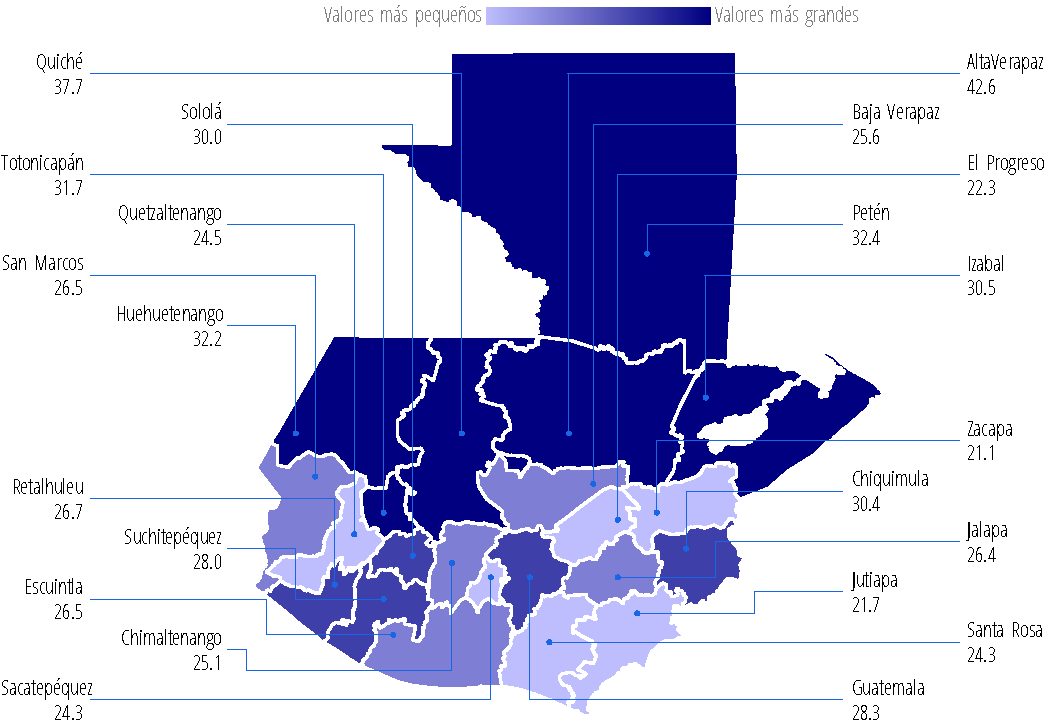
\includegraphics[width=52\cuadri]{C:/Users/INE/Desktop/compendio_educacion/graficas/basicos/1_19.pdf}}{Instituto Nacional de Estadística}





\cajita{Deserción}{La tasa de deserción en básico, presentó en el año 2009 el 8.2\% y en el año 2013 fue de 5.9\%, presentando un decrecimiento de 28.3\%.}{Tasa de deserción del ciclo de educación básica}{República de Guatemala, serie histórica, en porcentaje}{\ \\[0mm]\begin{tikzpicture}[x=1pt,y=1pt]  % Created by tikzDevice version 0.7.0 on 2015-08-31 18:35:32
% !TEX encoding = UTF-8 Unicode
\definecolor[named]{fillColor}{rgb}{1.00,1.00,1.00}
\path[use as bounding box,fill=fillColor,fill opacity=0.00] (0,0) rectangle (289.08,198.74);
\begin{scope}
\path[clip] (  0.00,  0.00) rectangle (289.08,198.74);
\definecolor[named]{drawColor}{rgb}{1.00,1.00,1.00}

\path[draw=drawColor,line width= 0.6pt,line join=round,line cap=round] (  0.00,  0.00) rectangle (289.08,198.74);
\end{scope}
\begin{scope}
\path[clip] (  0.00,  0.00) rectangle (289.08,198.74);

\path[] (  1.64, 17.78) rectangle (280.54,191.48);

\path[] (  1.64, 48.89) --
	(280.54, 48.89);

\path[] (  1.64, 95.34) --
	(280.54, 95.34);

\path[] (  1.64,141.79) --
	(280.54,141.79);

\path[] (  1.64,188.23) --
	(280.54,188.23);

\path[] (  1.64, 25.67) --
	(280.54, 25.67);

\path[] (  1.64, 72.12) --
	(280.54, 72.12);

\path[] (  1.64,118.56) --
	(280.54,118.56);

\path[] (  1.64,165.01) --
	(280.54,165.01);

\path[] ( 33.83, 17.78) --
	( 33.83,191.48);

\path[] ( 87.46, 17.78) --
	( 87.46,191.48);

\path[] (141.09, 17.78) --
	(141.09,191.48);

\path[] (194.73, 17.78) --
	(194.73,191.48);

\path[] (248.36, 17.78) --
	(248.36,191.48);
\definecolor[named]{drawColor}{rgb}{0.00,0.00,1.00}

\path[draw=drawColor,line width= 1.7pt,line join=round] ( 33.83,132.50) --
	( 87.46,183.59) --
	(141.09,114.85) --
	(194.73,103.70) --
	(248.36, 89.77);
\definecolor[named]{drawColor}{rgb}{0.00,0.00,0.00}

\node[text=drawColor,anchor=base,inner sep=0pt, outer sep=0pt, scale=  1.01] at ( 33.83,120.63) {6.5};

\node[text=drawColor,anchor=base,inner sep=0pt, outer sep=0pt, scale=  1.01] at ( 87.46,187.54) {12.0};

\node[text=drawColor,anchor=base west,inner sep=0pt, outer sep=0pt, scale=  1.01] at (141.09,118.80) {4.6};

\node[text=drawColor,anchor=base west,inner sep=0pt, outer sep=0pt, scale=  1.01] at (194.73,107.66) {3.4};

\node[text=drawColor,anchor=base,inner sep=0pt, outer sep=0pt, scale=  1.01] at (248.36, 77.90) {1.9};
\definecolor[named]{fillColor}{rgb}{0.00,0.00,0.00}

\path[draw=drawColor,line width= 0.1pt,line join=round,fill=fillColor] (  1.64, 25.67) -- (280.54, 25.67);
\end{scope}
\begin{scope}
\path[clip] (  0.00,  0.00) rectangle (289.08,198.74);

\path[] (  1.64, 17.78) --
	(  1.64,191.48);
\end{scope}
\begin{scope}
\path[clip] (  0.00,  0.00) rectangle (289.08,198.74);

\path[] (  0.00, 25.67) --
	(  1.64, 25.67);

\path[] (  0.00, 72.12) --
	(  1.64, 72.12);

\path[] (  0.00,118.56) --
	(  1.64,118.56);

\path[] (  0.00,165.01) --
	(  1.64,165.01);
\end{scope}
\begin{scope}
\path[clip] (  0.00,  0.00) rectangle (289.08,198.74);

\path[] (  1.64, 17.78) --
	(280.54, 17.78);
\end{scope}
\begin{scope}
\path[clip] (  0.00,  0.00) rectangle (289.08,198.74);

\path[] ( 33.83, 13.51) --
	( 33.83, 17.78);

\path[] ( 87.46, 13.51) --
	( 87.46, 17.78);

\path[] (141.09, 13.51) --
	(141.09, 17.78);

\path[] (194.73, 13.51) --
	(194.73, 17.78);

\path[] (248.36, 13.51) --
	(248.36, 17.78);
\end{scope}
\begin{scope}
\path[clip] (  0.00,  0.00) rectangle (289.08,198.74);
\definecolor[named]{drawColor}{rgb}{0.00,0.00,0.00}

\node[text=drawColor,anchor=base,inner sep=0pt, outer sep=0pt, scale=  1.00] at ( 33.83,  2.85) {2009};

\node[text=drawColor,anchor=base,inner sep=0pt, outer sep=0pt, scale=  1.00] at ( 87.46,  2.85) {2010};

\node[text=drawColor,anchor=base,inner sep=0pt, outer sep=0pt, scale=  1.00] at (141.09,  2.85) {2011};

\node[text=drawColor,anchor=base,inner sep=0pt, outer sep=0pt, scale=  1.00] at (194.73,  2.85) {2012};

\node[text=drawColor,anchor=base,inner sep=0pt, outer sep=0pt, scale=  1.00] at (248.36,  2.85) {2013};
\end{scope}
  \end{tikzpicture}}{Instituto Nacional de Estadística}

\cajita{Deserción por sexo}{La tasa de deserción en básico por sexo, representa el 7.1\% para hombres y 4.5\% para las mujeres.}{Tasa de deserción del ciclo de educación básica, por sexo}{República de Guatemala, año 2013, en porcentaje}{\ \\[0mm]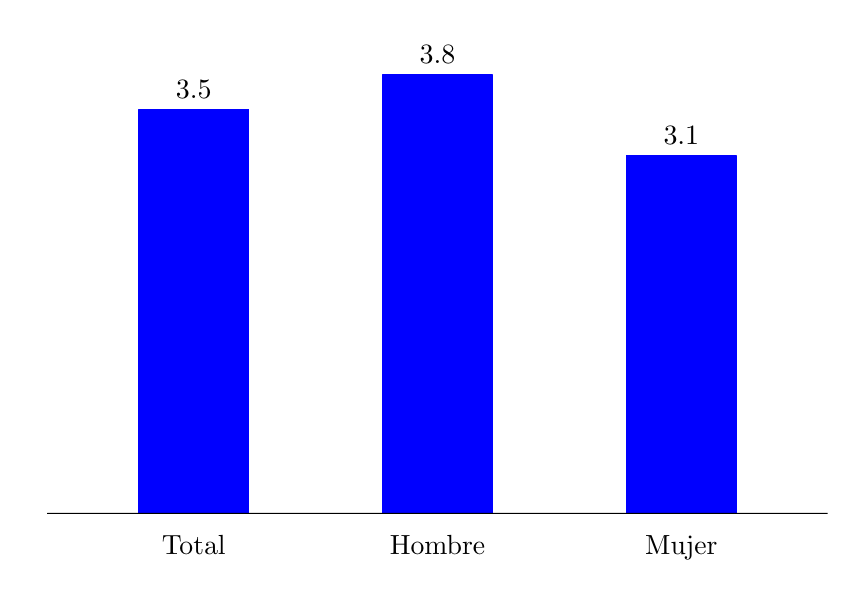
\begin{tikzpicture}[x=1pt,y=1pt]  % Created by tikzDevice version 0.7.0 on 2015-08-28 13:08:03
% !TEX encoding = UTF-8 Unicode
\definecolor[named]{fillColor}{rgb}{1.00,1.00,1.00}
\path[use as bounding box,fill=fillColor,fill opacity=0.00] (0,0) rectangle (289.08,198.74);
\begin{scope}
\path[clip] (  0.00,  0.00) rectangle (289.08,198.74);
\definecolor[named]{drawColor}{rgb}{1.00,1.00,1.00}

\path[draw=drawColor,line width= 0.6pt,line join=round,line cap=round] (  0.00,  0.00) rectangle (289.08,198.74);
\end{scope}
\begin{scope}
\path[clip] (  0.00,  0.00) rectangle (289.08,198.74);

\path[] (  7.11, 23.47) rectangle (289.08,181.67);

\path[] ( 59.98, 23.47) --
	( 59.98,181.67);

\path[] (148.10, 23.47) --
	(148.10,181.67);

\path[] (236.21, 23.47) --
	(236.21,181.67);
\definecolor[named]{drawColor}{rgb}{0.00,0.00,1.00}
\definecolor[named]{fillColor}{rgb}{0.00,0.00,1.00}

\path[draw=drawColor,line width= 0.6pt,line join=round,fill=fillColor] ( 40.16, 23.47) rectangle ( 79.81,169.18);

\path[draw=drawColor,line width= 0.6pt,line join=round,fill=fillColor] (128.27, 23.47) rectangle (167.92,181.67);

\path[draw=drawColor,line width= 0.6pt,line join=round,fill=fillColor] (216.39, 23.47) rectangle (256.04,152.53);
\definecolor[named]{drawColor}{rgb}{0.00,0.00,0.00}
\definecolor[named]{fillColor}{rgb}{0.00,0.00,0.00}

\path[draw=drawColor,line width= 0.1pt,line join=round,fill=fillColor] (  7.11, 23.47) -- (289.08, 23.47);

\node[text=drawColor,anchor=base,inner sep=0pt, outer sep=0pt, scale=  1.01] at ( 59.98,173.14) {3.5};

\node[text=drawColor,anchor=base,inner sep=0pt, outer sep=0pt, scale=  1.01] at (148.10,185.63) {3.8};

\node[text=drawColor,anchor=base,inner sep=0pt, outer sep=0pt, scale=  1.01] at (236.21,156.48) {3.1};
\end{scope}
\begin{scope}
\path[clip] (  0.00,  0.00) rectangle (289.08,198.74);

\path[] (  7.11, 23.47) --
	(  7.11,181.67);
\end{scope}
\begin{scope}
\path[clip] (  0.00,  0.00) rectangle (289.08,198.74);

\path[] (  7.11, 23.47) --
	(289.08, 23.47);
\end{scope}
\begin{scope}
\path[clip] (  0.00,  0.00) rectangle (289.08,198.74);

\path[] ( 59.98, 19.20) --
	( 59.98, 23.47);

\path[] (148.10, 19.20) --
	(148.10, 23.47);

\path[] (236.21, 19.20) --
	(236.21, 23.47);
\end{scope}
\begin{scope}
\path[clip] (  0.00,  0.00) rectangle (289.08,198.74);
\definecolor[named]{drawColor}{rgb}{0.00,0.00,0.00}

\node[text=drawColor,anchor=base,inner sep=0pt, outer sep=0pt, scale=  1.00] at ( 59.98,  8.54) {Total};

\node[text=drawColor,anchor=base,inner sep=0pt, outer sep=0pt, scale=  1.00] at (148.10,  8.54) {Hombre};

\node[text=drawColor,anchor=base,inner sep=0pt, outer sep=0pt, scale=  1.00] at (236.21,  8.54) {Mujer};
\end{scope}
  \end{tikzpicture}}{Instituto Nacional de Estadística}

\cajota{Deserción en los departamentos}{En el siguiente mapa se observan los departamentos donde hubo baja tasa de deserción en básico: Jutiapa 4.2\%, Chimaltenango 4.5\% y Quetzaltenango 4.9\%.\\ 
	
	 Los departamentos donde hubo alta tasa  de deserción en básico: Santa Rosa 9.5\%, Retalhuleu 9.6\% e Izabal 10.4\%. En el departamento de Guatemala la tasa de deserción fue de 7.8\%.	}{Tasa de deserción del ciclo de educación básica}{Por departamento, año 2013, en porcentaje}{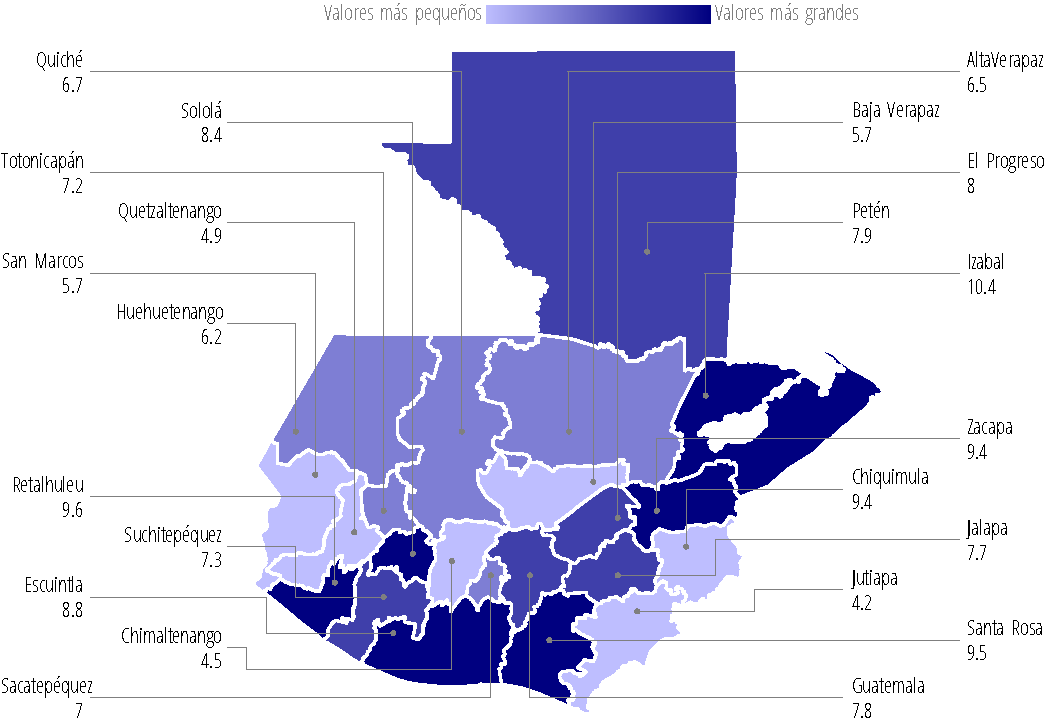
\includegraphics[width=52\cuadri]{C:/Users/INE/Desktop/compendio_educacion/graficas/basicos/1_22.pdf}}{Instituto Nacional de Estadística}




\cajita{Aprobación}{La tasa de aprobación en básico, presentó el año 2009 el 68.4\% y en el año 2013 fue de 69.6\%, presentando un crecimiento de 1.7\%.}{Tasa de aprobación del ciclo de educación básica}{República de Guatemala, serie histórica, en porcentaje}{\ \\[0mm]\begin{tikzpicture}[x=1pt,y=1pt]  % Created by tikzDevice version 0.7.0 on 2015-08-28 13:08:13
% !TEX encoding = UTF-8 Unicode
\definecolor[named]{fillColor}{rgb}{1.00,1.00,1.00}
\path[use as bounding box,fill=fillColor,fill opacity=0.00] (0,0) rectangle (289.08,198.74);
\begin{scope}
\path[clip] (  0.00,  0.00) rectangle (289.08,198.74);
\definecolor[named]{drawColor}{rgb}{1.00,1.00,1.00}

\path[draw=drawColor,line width= 0.6pt,line join=round,line cap=round] (  0.00,  0.00) rectangle (289.08,198.74);
\end{scope}
\begin{scope}
\path[clip] (  0.00,  0.00) rectangle (289.08,198.74);

\path[] (  1.64, 17.78) rectangle (280.54,191.48);

\path[] (  1.64, 55.35) --
	(280.54, 55.35);

\path[] (  1.64,114.72) --
	(280.54,114.72);

\path[] (  1.64,174.09) --
	(280.54,174.09);

\path[] (  1.64, 25.67) --
	(280.54, 25.67);

\path[] (  1.64, 85.04) --
	(280.54, 85.04);

\path[] (  1.64,144.41) --
	(280.54,144.41);

\path[] ( 33.83, 17.78) --
	( 33.83,191.48);

\path[] ( 87.46, 17.78) --
	( 87.46,191.48);

\path[] (141.09, 17.78) --
	(141.09,191.48);

\path[] (194.73, 17.78) --
	(194.73,191.48);

\path[] (248.36, 17.78) --
	(248.36,191.48);
\definecolor[named]{drawColor}{rgb}{0.00,0.00,1.00}

\path[draw=drawColor,line width= 1.7pt,line join=round] ( 33.83,182.40) --
	( 87.46,174.68) --
	(141.09,172.90) --
	(194.73,178.24) --
	(248.36,183.59);
\definecolor[named]{drawColor}{rgb}{0.00,0.00,0.00}

\node[text=drawColor,anchor=base,inner sep=0pt, outer sep=0pt, scale=  1.01] at ( 33.83,186.36) {86.4};

\node[text=drawColor,anchor=base west,inner sep=0pt, outer sep=0pt, scale=  1.01] at ( 87.46,178.64) {85.1};

\node[text=drawColor,anchor=base,inner sep=0pt, outer sep=0pt, scale=  1.01] at (141.09,161.03) {84.8};

\node[text=drawColor,anchor=base east,inner sep=0pt, outer sep=0pt, scale=  1.01] at (191.61,178.24) {85.7};

\node[text=drawColor,anchor=base,inner sep=0pt, outer sep=0pt, scale=  1.01] at (248.36,187.54) {86.6};
\definecolor[named]{fillColor}{rgb}{0.00,0.00,0.00}

\path[draw=drawColor,line width= 0.1pt,line join=round,fill=fillColor] (  1.64, 25.67) -- (280.54, 25.67);
\end{scope}
\begin{scope}
\path[clip] (  0.00,  0.00) rectangle (289.08,198.74);

\path[] (  1.64, 17.78) --
	(  1.64,191.48);
\end{scope}
\begin{scope}
\path[clip] (  0.00,  0.00) rectangle (289.08,198.74);

\path[] (  0.00, 25.67) --
	(  1.64, 25.67);

\path[] (  0.00, 85.04) --
	(  1.64, 85.04);

\path[] (  0.00,144.41) --
	(  1.64,144.41);
\end{scope}
\begin{scope}
\path[clip] (  0.00,  0.00) rectangle (289.08,198.74);

\path[] (  1.64, 17.78) --
	(280.54, 17.78);
\end{scope}
\begin{scope}
\path[clip] (  0.00,  0.00) rectangle (289.08,198.74);

\path[] ( 33.83, 13.51) --
	( 33.83, 17.78);

\path[] ( 87.46, 13.51) --
	( 87.46, 17.78);

\path[] (141.09, 13.51) --
	(141.09, 17.78);

\path[] (194.73, 13.51) --
	(194.73, 17.78);

\path[] (248.36, 13.51) --
	(248.36, 17.78);
\end{scope}
\begin{scope}
\path[clip] (  0.00,  0.00) rectangle (289.08,198.74);
\definecolor[named]{drawColor}{rgb}{0.00,0.00,0.00}

\node[text=drawColor,anchor=base,inner sep=0pt, outer sep=0pt, scale=  1.00] at ( 33.83,  2.85) {2009};

\node[text=drawColor,anchor=base,inner sep=0pt, outer sep=0pt, scale=  1.00] at ( 87.46,  2.85) {2010};

\node[text=drawColor,anchor=base,inner sep=0pt, outer sep=0pt, scale=  1.00] at (141.09,  2.85) {2011};

\node[text=drawColor,anchor=base,inner sep=0pt, outer sep=0pt, scale=  1.00] at (194.73,  2.85) {2012};

\node[text=drawColor,anchor=base,inner sep=0pt, outer sep=0pt, scale=  1.00] at (248.36,  2.85) {2013};
\end{scope}
  \end{tikzpicture}}{Instituto Nacional de Estadística}

\cajita{Aprobación por sexo}{La tasa de aprobación en básico por sexo, representa el 66\% para hombres y 73.6\% para las mujeres.}{Tasa de aprobación del ciclo de educación básica, por sexo}{República de Guatemala, año 2013, en porcentaje}{\ \\[0mm]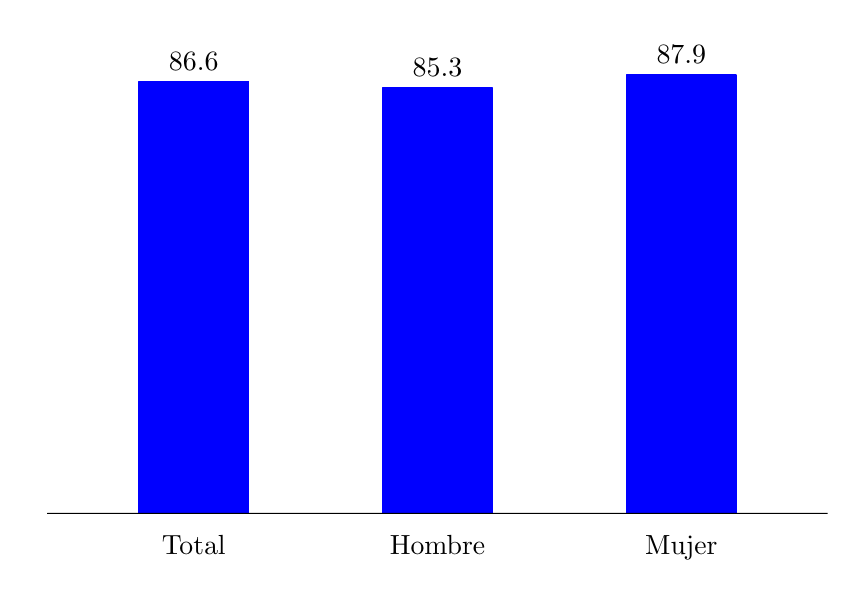
\begin{tikzpicture}[x=1pt,y=1pt]  % Created by tikzDevice version 0.7.0 on 2015-08-28 13:08:16
% !TEX encoding = UTF-8 Unicode
\definecolor[named]{fillColor}{rgb}{1.00,1.00,1.00}
\path[use as bounding box,fill=fillColor,fill opacity=0.00] (0,0) rectangle (289.08,198.74);
\begin{scope}
\path[clip] (  0.00,  0.00) rectangle (289.08,198.74);
\definecolor[named]{drawColor}{rgb}{1.00,1.00,1.00}

\path[draw=drawColor,line width= 0.6pt,line join=round,line cap=round] (  0.00,  0.00) rectangle (289.08,198.74);
\end{scope}
\begin{scope}
\path[clip] (  0.00,  0.00) rectangle (289.08,198.74);

\path[] (  7.11, 23.47) rectangle (289.08,181.67);

\path[] ( 59.98, 23.47) --
	( 59.98,181.67);

\path[] (148.10, 23.47) --
	(148.10,181.67);

\path[] (236.21, 23.47) --
	(236.21,181.67);
\definecolor[named]{drawColor}{rgb}{0.00,0.00,1.00}
\definecolor[named]{fillColor}{rgb}{0.00,0.00,1.00}

\path[draw=drawColor,line width= 0.6pt,line join=round,fill=fillColor] ( 40.16, 23.47) rectangle ( 79.81,179.33);

\path[draw=drawColor,line width= 0.6pt,line join=round,fill=fillColor] (128.27, 23.47) rectangle (167.92,176.99);

\path[draw=drawColor,line width= 0.6pt,line join=round,fill=fillColor] (216.39, 23.47) rectangle (256.04,181.67);
\definecolor[named]{drawColor}{rgb}{0.00,0.00,0.00}
\definecolor[named]{fillColor}{rgb}{0.00,0.00,0.00}

\path[draw=drawColor,line width= 0.1pt,line join=round,fill=fillColor] (  7.11, 23.47) -- (289.08, 23.47);

\node[text=drawColor,anchor=base,inner sep=0pt, outer sep=0pt, scale=  1.01] at ( 59.98,183.29) {86.6};

\node[text=drawColor,anchor=base,inner sep=0pt, outer sep=0pt, scale=  1.01] at (148.10,180.95) {85.3};

\node[text=drawColor,anchor=base,inner sep=0pt, outer sep=0pt, scale=  1.01] at (236.21,185.63) {87.9};
\end{scope}
\begin{scope}
\path[clip] (  0.00,  0.00) rectangle (289.08,198.74);

\path[] (  7.11, 23.47) --
	(  7.11,181.67);
\end{scope}
\begin{scope}
\path[clip] (  0.00,  0.00) rectangle (289.08,198.74);

\path[] (  7.11, 23.47) --
	(289.08, 23.47);
\end{scope}
\begin{scope}
\path[clip] (  0.00,  0.00) rectangle (289.08,198.74);

\path[] ( 59.98, 19.20) --
	( 59.98, 23.47);

\path[] (148.10, 19.20) --
	(148.10, 23.47);

\path[] (236.21, 19.20) --
	(236.21, 23.47);
\end{scope}
\begin{scope}
\path[clip] (  0.00,  0.00) rectangle (289.08,198.74);
\definecolor[named]{drawColor}{rgb}{0.00,0.00,0.00}

\node[text=drawColor,anchor=base,inner sep=0pt, outer sep=0pt, scale=  1.00] at ( 59.98,  8.54) {Total};

\node[text=drawColor,anchor=base,inner sep=0pt, outer sep=0pt, scale=  1.00] at (148.10,  8.54) {Hombre};

\node[text=drawColor,anchor=base,inner sep=0pt, outer sep=0pt, scale=  1.00] at (236.21,  8.54) {Mujer};
\end{scope}
  \end{tikzpicture}}{Instituto Nacional de Estadística}

\cajota{Aprobación en los departamentos}{En el siguiente mapa se observan los departamentos donde hubo baja tasa de aprobación en básico: Sacatepéquez 60.8\%, Quetzaltenango 61.5\% y Chimaltenango 63.9\%. \\ 
	
	 Los departamentos donde hubo alta tasa  de aprobación en básico fueron: Chiquimula 76.8\% Jalapa 76.9\% y Petén 77.1\%. El departamento de Guatemala presentó una tasa de aprobación de 68.5\%.}{Tasa de aprobación del ciclo de educación básica}{Por departamento, año 2013, en porcentaje}{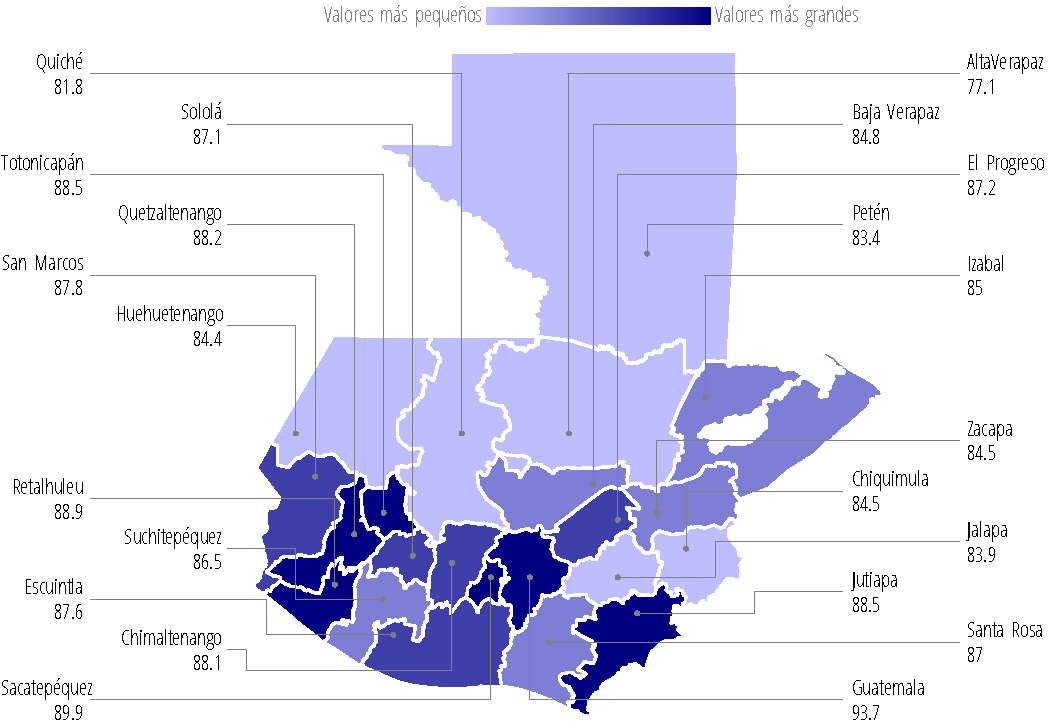
\includegraphics[width=52\cuadri]{C:/Users/INE/Desktop/compendio_educacion/graficas/basicos/1_25.pdf}}{Instituto Nacional de Estadística}



